\documentclass[11pt]{scrartcl}
 
 \usepackage{graphicx}
\usepackage{scrlayer-scrpage}
\usepackage{listings }
\usepackage{hyperref}
\usepackage{listingsutf8}
\usepackage{subfigure}
\pagestyle{scrheadings}
\clearscrheadfoot
\ifoot[]{\author}
\ofoot[]{\pagemark} 
 \title{Optimierung von Trainingsdaten für semantische Segmentierung}
\author{Christopher Pasda}
\usepackage{float}
\restylefloat{figure}


\begin{document}
\maketitle
\tableofcontents

\newpage

\section{Einleitung}
\label{sec:Einleitung}

\noindent
Seit Anbeginn der digitalen Revolution Ende des 20 Jahrhunderts hat sich unsere Welt grundlegend verändert. Mit dem technologischen Fortschritt wurde nicht nur die Hardware kleiner und leistungsfähiger, auch die Software wurde intelligenter und benutzerfreundlicher. Die Spitze der technologischen Errungenschaften der letzten Jahre stellen heute Neuronale Netzwerke dar, welche für einen bestimmten Zweck trainiert werden können. So wird versucht sich immer wiederholende Prozesse durch künstliche Intelligenzen zu steuern. Dazu gehört auch das autonome Fahren. Der technologische-Wettbewerb in diesem Bereich ist in vollem Gange, was sich dadurch zeigt, dass große Firmen in den letzten Jahren  sehr viel Geld investierten. Es liegt auf der Hand, dass diese Technologien auch in anderen Bereichen, wie zum Beispiel der Schienenerkennung, von großem Nutzen sind. 
Für das Forschungsprojekt von Prof. Dr.-Ing. Carsten Thomas in Zusammenarbeit mit der Firma BOSCH Engineering zum Thema "Digitale Schiene", soll der Prozess der Erstellung von Trainingsdaten für die semantische Segmentierung optimiert werden, damit auch eigene Trainingsdaten erstellt werden können. Dies ist notwendig, da existierende Datensätze nicht für kommerzielle Zwecke verwendet werden können. Ziel der Arbeit ist die Entwicklung eines Prototyps, welcher den Prozess des Labelns\footnote{Labeln beschreibt den Prozess, bei dem jeder Klasse eines Bildes verschiedene Farbcodes zugeordnet werden, um sie so unterscheiden zu können.} eines Bildes optimiert. Weiterhin sollen Daten für Benchmarks und                                                                                                                                                                                                                                                                                                                                                                                                                                                                                                                                                                                                                                                                                                                                                                                                                                                                                                                                                                                                                                                                                                                                                                                                                                                                                                                                                                                                                                                                                                                                                                                                                                                                                                                                                                                                                                                                                                                                                                                                                                                                                                                                                                                                                                                                                                                                                                                                                                                                                                                                                                                                                                                                                                                                                                                                                                                                                                                                                                                                                                                                                                                                                                                                                                                                                                                                                                                                                                                                                                                                                                                                                                                                                                                                                                                                                                                                                                                                                                                                                                                                                                                                                                                                                                                                                                                                                                                                                                                                                                                                                                                                                                                                                                                                                                                                                                                                                                                                                                                                                                                                                                                                                                                                                                                                                                                                                                                                                                                                                                                                                                                                                                                                                                                                                                                                                                                                                                                                                                                                                                                                                                                                                                                                                                                                                                                                                                                                                                                                                                                                                                                                                                                                                                                                                                                                                                                                                                                                                                                                                                                                                                                                                                                                                                                                                                                                                                                                                                                                                                                                                                                                                                                                                                                                                                                                                                                                                                                                                                                                                                                                                                                                                                                                                                                                                                                                                                                                                                                                                                                                                                                                                                                                                                                                                                                                                                                                                                                                                                                                                                                                                                                                                                                                                                                                                                                                                                                                                                                                                                                                                                                                                                                                                                                                                                                                                                                                                                                                                                                                                                                                                                                                                                                                                                                                                                                                                                                                                                                                                                                                                                                                                                                                                                                                                                                                                                                                                                                                                                                                                                                                                                                                                                                                                                                                                                                                                                                                                                                                                                                                                                                                                                                                                                                                                                                                                                                                                                                                                                                                                                                                                                                                                                                                                                                                                                                                                                                                                                                                                                                                                                                                                                                                                                                                                                                                                                                                                                                                                                                                                                                                                                                                                                                                                                                                                                                                                                                                                                                                                                                                                                                                                                                                                                                                                                                                                                                                                                                                                                                                                                                                                                                                                                                                                                                                                                                                                                                                                                                                                                                                                                                                                                                                                                                                                                                                                                                                                                                                                                                                                                                                                                                                                                                                                                                                                                                                                                                                                                                                                                                                                                                                                                                                                                                                                                                                                                                                                                                                                                                                                                                                                                                                                                                                                                                                                                                                                                                                                                                                                                                                                                                                                                                                                                                                                                                                                                                                                                                                                                                                                                                                                                                                                                                                                                                                                                                                                                                                                                                                                                                                                                                                                                                                                                                                                                                                                                                                                                                                                                                                                                                                                                                                                                                                                                                                                                                                                                                                                                                                                                                                                                                                                                                                                                                                                                                                                                                                                                                                                                                                                                                                                                                                                                                                                                                                                                                                                                                                                                                                                                                                                                                                                                                                                                                                                                                                                                                                                                                                                                                                                                                                                                                                                                                                                                                                                                                                                                                                                                                                                                                                                                                                                                                                                                                                                                                                                                                                                                                                                                                                                                                                                                                                                                                                                                                                                                                                                                                                                                                                                                                                                                                                                                                                                                                                                                                                                                                                                                                                                                                                                                                                                                                                                                                                                                                                                                                                                                                                                                                                                                                                                                                                                                                                                                                                                                                                                                                                                                                                                                                                                                                                                                                                                                                                                                                                                                                                                                                                                                                                                                                                                                                                                                                                                                                                                                                                                                                                                                                                                                                                                                                                                                                                                                                                                                                                                                                                                                                                                                                                                                                                                                                                                                                                                                                                                                                                                                                                                                                                                                                                                                                                                                                                                                                                                                                                                                                                                                                                                                                                                                                                                                                                                                                                                                                                                                                                                                                                                                                                                                                                                                                                                                                                                                                                                                                                                                                                                                                                                                                                                                                                                                                                                                                                                                                                                                                                                                                                                                                                                                                                                                                                                                                                                                                                                                                                                                                                                                                                                                                                                                                                                                                                                                                                                                                                                                                                                                                                                                                                                                                                                                                                                                                                                                                                                                                                                                                                                                                                                                                                                                                                                                                                                                                                                                                                                                                                                                                                                                                                                                                                                                                                                                                                                                                                                                                                                                                                                                                                                                                                                                                                                                                                                                                                                                                                                                                                                                                                                                                                                                                                                                                                                                                                                                                                                                                                                                                                                                                                                                                                                                                                                                                                                                                                                                                                                                                                                                                                                                                                                                                                                                                                                                                                                                                                                                                                                                                                                                                                                                                                                                                                                                                                                                                                                                                                                                                                                                                                                                                                                                                                                                                                                                                                                                                                                                                                                                                                                                                                                                                                                                                                                                                                                                                                                                                                                                                                                                                                                                                                                                                                                                                                                                                                                                                                                                                                                                                                                                                                                                                                                                                                                                                                                                                                                                                                                                                                                                                                                                                                                                                                                                                                                                                                                                                                                                                                                                                                                                                                                                                                                                                                                                                                                                                                                                                                                                                                                                                                                                                                                                                                                                                                                                                                                                                                                                                                                                                                                                                                                                                                                                                                                                                                                                                                                                                                                                                                                                                                                                                                                                                                                                                                                                                                                                                                                                                                                                                                                                                                                                                                                                                                                                                                                                                                                                                                                                                                                                                                                                                                                                                                                                                                                                                                                                                                                                                                                                                                                                                                                                                                                                                                                                                                                                                                                                                                                                                                                                                                                                                                                                                                                                                                                                                                                                                                                                                                                                                                                                                                                                                                                                                                                                                                                                                                                                                                                                                                                                                                                                                                                                                                                                                                                                                                                                                                                                                                                                                                                                                                                                                                                                                                                                                                                                                                                                                                                                                                                                                                                                                                                                                                                                                                                                                                                                                                                                                                                                                                                                                                                                                                                                                                                                                                                                                                                                                                                                                                                                                                                                                                                                                                                                                                                                                                                                                                                                                                                                                                                                                                                                                                                                                                                                                                                                                                                                                                                                                                                                                                                                                                                                                                                                                                                                                                                                                                                                                                                                                                                                                                                                                                                                                                                                                                                                                                                                                                                                                                                                                                                                                                                                                                                                                                                                                                                                                                                                                                                                                                                                                                                                                                                                                                                                                                                                                                                                                                                                                                                                                                                                                                                                                                                                                                                                                                                                                                                                                                                                                                                                                                                                                                                                                                                                                                                                                                                                                                                                                                                                                                                                                                                                                                                                                                                                                                                                                                                                                                                                                                                                                                                                                                                                                                                                                                                                                                                                                                                                                                                                                                                                                                                                                                                                                                                                                                                                                                                                                                                                                                                                                                                                                                                                                                                                                                                                                                                                                                                                                                                                                                                                                                                                                                                                                                                                                                                                                                                                                                                                                                                                                                                                                                                                                                                                                                                                                                                                                                                                                                                                                                                                                                                                                                                                                                                                                                                                                                                                                                                                                                                                                                                                                                                                                                                                                                                                                                                                                                                                                                                                                                                                                                                                                                                                                                                                                                                                                                                                                                                                                                                                                                                                                                                                                                                                                                                                                                                                                                                                                                                                                                                                                                                                                                                                                                                                                                                                                                                                                                                                                                                                                                                                                                                                                                                                                                                                                                                                                                                                                                                                                                                                                                                                                                                                                                                                                                                                                                                                                                                                                                                                                                                                                                                                                                                                                                                                                                                                                                                                                                                                                                                                                                                                                                                                                                                                                                                                                                                                                                                                                                                                                                                                                                                                                                                                                                                                                                                                                                                                                                                                                                                                                                                                                                                                                                                                                                                                                                                                                                                                                                                                                                                                                                                                                                                                                                                                                                                                                                                                                                                                                                                                                                                                                                                                                                                                                                                                                                                                                                                                                                                                                                                                                                                                                                                                                                                                                                                                                                                                                                                                                                                                                                                                                                                                                                                                                                                                                                                                                                                                                                                                                                                                                                                                                                                                                                                                                                                                                                                                                                                                                                                                                                                                                                                                                                                                                                                                                                                                                                                                                                                                                                                                                                                                                                                                                                                                                                                                                                                                                                                                                                                                                                                                                                                                                                                                                                                                                                                                                                                                                                                                                                                                                                                                                                                                                                                                                                                                                                                                                                                                                                                                                                                                                                                                                                                                                                                                                                                                                                                                                                                                                                                                                                                                                                                                                                                                                                                                                                                                                                                                                                                                                                                                                                                                                                                                                                                                                                                                                                                                                                                                                                                                                                                                                                                                                                                                                                                                                                                                                                                                                                                                                                                                                                                                                                                                                                                                                                                                                                                                                                                                                                                                                                                                                                                                                                                                                                                                                                                                                                                                                                                                                                                                                                                                                                                                                                                                                                                                                                                                                                                                                                                                                                                                                                                                                                                                                                                                                                                                                                                                                                                                                                                                                                                                                                                                                                                                                                                                                                                                                                                                                                                                                                                                                                                                                                                                                                                                                                                                                                                                                                                                                                                                                                                                                                                                                                                                                                                                                                                                                                                                                                                                                                                                                                                                                                                                                                                                                                                                                                                                                                                                                                                                                                                                                                                                                                                                                                                                                                                                                                                                                                                                                                                                                                                                                                                                                                                                                                                                                                                                                                                                                                                                                                                                                                                                                                                                                                                                                                                                                                                                                                                                                                                                                                                                                                                                                                                                                                                                                                                                                                                                                                                                                                                                                                                                                                                                                                                                                                                                                                                                                                                                                                                                                                                                                                                                                                                                                                                                                                                                                                                                                                                                                                                                                                                                                                                                                                                                                                                                                                                                                                                                                                                                                                                                                                                                                                                                                                                                                                                                                                                                                                                                                                                                                                                                                                                                                                                                                                                                                                                                                                                                                                                                                                                                                                                                                                                                                                                                                                                                                                                                                                                                                                                                                                                                                                                                                                                                                                                                                                                                                                                                                                                                                                                                                                                                                                                                                                                                                                                                                                                                                                                                                                                                                                                                                                                                                                                                                                                                                                                                                                                                                                                                                                                                                                                                                                                                                                                                                                                                                                                                                                                                                                                                                                                                                                                                                                                                                                                                                                                                                                                                                                                                                                                                                                                                                                                                                                                                                                                                                                                                                                                                                                                                                                                                                                                                                                                                                                                                                                                                                                                                                                                                                                                                                                                                                                                                                                                                                                                                                                                                                                                                                                                                                                                                                                                                                                                                                                                                                                                                                                                                                                                                                                                                                                                                                                                                                                                                                                                                                                                                                                                                                                                                                                                                                                                                                                                                                                                                                                                                                                                                                                                                                                                                                                                                                                                                                                                                                                                                                                                                                                                                                                                                                                                                                                                                                                                                                                                                                                                                                                                                                                                                                                                                                                                                                                                                                                                                                                                                                                                                                                                                                                                                                                                                                                                                                                                                                                                                                                                                                                                                                                                                                                                                                                                                                                                                                                                                                                                                                                                                                                                                                                                                                                                                                                                                                                                                                                                                                                                                                                                                                                                                                                                                                                                                                                                                                                                                                                                                                                                                                                                                                                                                                                                                                                                                                                                                                                                                                                                                                                                                                                                                                                                                                                                                                                                                                                                                                                                                                                                                                                                                                                                                                                                                                                                                                                                                                                                                                                                                                                                                                                                                                                                                                                                                                                                                                                                                                                                                                                                                                                                                                                                                                                                                                                                                                                                                                                                                                                                                                                                                                                                                                                                                                                                                                                                                                                                                                                                                                                                                                                                                                                                                                                                                                                                                                                                                                                                                                                                                                                                                                                                                                                                                                                                                                                                                                                                                                                                                                                                                                                                                                                                                                                                                                                                                                                                                                                                                                                                                                                                                                                                                                                                                                                                                                                                                                                                                                                                                                                                                                                                                                                                                                                                                                                                                                                                                                                                                                                                                                                                                                                                                                                                                                                                                                                                                                                                                                                                                                                                                                                                                                                                                                                                                                                                                                                                                                                                                                                                                                                                                                                                                                                                                                                                                                                                                                                                                                                                                                                                                                                                                                                                                                                                                                                                                                                                                                                                                                                                                                                                                                                                                                                                                                                                                                                                                                                                                                                                                                                                                                                                                                                                                                                                                                                                                                                                                                                                                                                                                                                                                                                                                                                                                                                                                                                                                                                                                                                                                                                                                                                                                                                                                                                                                                                                                                                                                                                                                                                                                                                                                                                                                                                                                                                                                                                                                                                                                                                                                                                                                                                                                                                                                                                                                                                                                                                                                                                                                                                                                                                                                                                                                                                                                                                                                                                                                                                                                                                                                                                                                                                                                                                                                                                                                                                                                                                                                                                                                                                                                                                                                                                                                                                                                                                                                                                                                                                                                                                                                                                                                                                                                                                                                                                                                                                                                                                                                                                                                                                                                                                                                                                                                                                                                      Performance-Analysen erhoben und vorhandene Label durch Drittanbieter erweitert werden können.
Im ersten Teil dieser Arbeit werden verschiedene Tools analysiert und dazu in einer Pro- und Contraliste visualisiert, inwiefern Funktionen und Features sich als nützlich erweisen können. Darauf aufbauend wird das "Annotation Tool" von Herrn Mario Hoffmann analysiert und  Anforderungen aus den Anwendungsdiagrammen abgeleitet. Im zweiten Teil wird das Programm, basierend auf einer Idee von Herr Thomas, vorgestellt und diskutiert. Abschließend folgt eine Qualitätskontrolle und das Fazit der Arbeit.


\newpage
\section{Projekt SE Perception}
\label{sec:Projekt SE Perception}

\subsection{Überblick}
\label{sec:Überblick}

\noindent
Die vorliegende Arbeit wurde im Zusammenhang des Projektes SE Perception zwischen der Hochschule für Technik und Wirtschaft Berlin und der Firma BOSCH Engineering realisiert. Das Ziel des Projektes legt den Fokus auf die automatische Erkennung von Schienen und Fahrwegen, wofür mehrere verschiedene Ansätze erforscht wurden. Einer dieser Ansatze stellt die Erkennung von Schienen mittels Algorithmen dar. Diese Algorithmen basieren auf der Möglichkeit ein Bild in eine sogenannte "Birdview" umzuwandeln. Das bedeutet, dass man durch Berechnungen eine direkte Sicht von oben auf die Schiene aus einem Bild erzeugen kann. Durch Vorverarbeitung und Kantenerkennung kann mittels des "Birdviews" die genaue Position einer Schiene im Bild bestimmt werden. Diese Sicht von oben wird im Ergebnis dazu genutzt Mittelpunkte zu generieren, welche den Verlauf der Schiene anzeigen sollen. Da die Erkennungsgüte jedoch sehr von der Qualität und Belichtung des vorliegenden Bildes abhängt, wurde in einem weiteren Ansatz versucht ein neuronales Netzwerk zur Schienenerkennung zu verwenden . Um ein solches Netzwerk effektiv nutzen zu können, muss dieses vorab trainiert werden. Dazu werden Beispielbilder, welche eine Abbildung der jeweiligen Situation die erkannt werden soll darstellen, entsprechend markiert und daraus Ground Truth Daten\footnote{Ground Truth eine gebräuchliche Terminologie, die in verschiedenen Bereichen häufig verwendet wird, um sich grundsätzlich auf jede Art von Information zu beziehen, die durch direkte Beobachtung bereitgestellt wird} erstellt. Das sind uint8\footnote{vorzeichenunbehafteter Integer mit 8 Bit-Informationen (0-255)}-Bilder, welche die Informationen über die jeweilige Klasse in einem Pixel gespeichert haben. Daraus entsteht ein Grauwert-Bild, welches Objekte in Bildern maschinenverständlich darstellen kann. Um solche Ground Truth Daten erstellen zu können, muss ein Bild vorher entsprechend markiert werden.  Dazu werden interessante Bereiche (ROI = region of interest) pixelweise in der jeweiligen Klassenfarbe markiert. So können die verschiedenen Objekte im Bild ihrer Klasse zugeorndet werden. Dies ist ein aufwändiger Prozess, welcher abhängig vom Bild bis zu einer Stunde dauern kann. Diese Informationen werden dazu verwendet das neuronale Netzwerk zu Trainieren. 

\begin{figure}[H]
  \includegraphics[width=1\textwidth]{bsp}
  \caption{Beispiel Overlay mit Pixelmaske}
\end{figure}
\noindent 
Aus diesen Pixelmasken können im nächsten Schritt Ground Truth Daten erstellt werden, mit denen ein neuronales Netzwerk auf die Erkennung der jeweiligen Klassen trainiert werden kann. Im Ergebnis kann durch eine "Heatmap"\footnote{Diagramm zur Visualisierung von Daten aufgrund einer Funktion, rot = Wahrscheinlichkeit der Erkennung hoch, blau = Wahrscheinlichkeit der Erkennung niedrig} gezeigt werden, mit welcher Wahrscheinlichkeit das Neuronale Netzwerk die Schienen erkennt. Dabei wird mittels eines ROS-Knoten eine Daten-Verbindung zwischen einem Video und dem Neuronalen Netzwerk geknüpft. Durch den Input des Videos in das Neuronale Netzwerk können die Informationen entsprechend verarbeitet und Schienen erkannt werden.
\begin{figure}[H]
  \includegraphics[width=1\textwidth]{netzwerk}
  \caption{Wahrscheinlich der Erkennung von Schienen durch das Netzwerk}
\end{figure}
\noindent 
Die Güte der Erkennung hängt dabei direkt von der Anzahl und Qualität der Trainingsdaten ab. Der momentan verwendete Datensatz  umfasst 8500 Bilder und äquivalent viele Labels. Davon werden circa 70\% für das Training und 30\% der Bilder für das Testen des Netzwerkes benötigt. Es wird deutlich, dass eine große Anzahl an Bildern für ein Training gebraucht wird. Neben diesen Informationen zum Training des Netzwerkes sollen noch Mittelpunkte und Pixel-Vektoren der Label erzeugt werden, damit diese von einem Drittanbieter gelesen und erweitert werden können. Die Mittelpunke werden vorrangig für Benchmarks der Algorithmen benötigt.
\\

\noindent
\textbf{Hauptziel:}
\\

\noindent
Das Hauptziel des Projektes stellt eine Kombination beider Ansätze dar, sodass ein neuronales Netzwerk dazu verwendet wird ein segmentiertes Bild zu erstellen, aus dem die Schiene gefiltert wird. Auf diesem binären Bild, welches nur noch die Schieneninformation trägt, sollen im Anschluss die Algortihmen zur Schienenerkennung angewendet werden. 
\begin{figure}[H]
  \includegraphics[width=1\textwidth]{einleitung}
  \caption{Hauptziel des Projektes}
\end{figure}
\noindent 
\subsection{Problemstellung}
\label{sec:Problemstellung}

Da die Erkennungsgüte des Netzwerks mit der Qualität der Trainingsbilder einhergeht, ist es notwendig Bilder möglichst akkurat zu markieren. Wie im späteren Verlauf beschrieben wird, gibt es  wenige unterstützende Softwarefunktionen, welche diesen Prozess beschleunigen können. So müssen Bilder momentan per Hand markiert werden, was einen sehr zeitaufwändigen Prozess darstellt und bei der Größe des benötigten Datensatzes kaum realisierbar scheint. So wurde in erster Instanz ein existierender Datensatz verwendet um das neuronale Netzwerk zu trainieren. Dabei handelt es sich um den "Railsem19" Datensatz\footnote{Datensatz vom Austrian Institute of Technology}, welcher jedoch nicht für kommerzielle Zwecke genutzt werden darf und dadruch an Bedeutung für dieses Projekt verliert.
Daraus entstand die Notwendigkeit für ein Programm, welches den Prozess des Labelns beschleunigt, um einen eigenen geeigneten Datensatz erstellen zu können. 

\subsection{Grundidee des Labeltools}
\label{sec:Grundidee des Labeltools}

Die Grundidee zu dieser Arbeit stammt von Prof. Dr.-Ing. Carsten Thomas. Im Kern geht es darum Mittelpunkte zwischen der linken und rechten Schiene zu verwenden, um daraus Label für die Schienen erstellen zu können. Realisiert werden kann dies durch die Umrechnung zwischen Pixel- und Weltkoordinaten. Verfeinert wurde die Grundidee von Prof. Dr. rer. nat. Frank Bauernöppel, welcher im späteren Verlauf die Verwendung eines Catmull-Rom Splines vorgeschlagen hat.  Dadurch lässt sich der Schienenverlauf sehr genau abbilden, da die Fuktion zwischen zwei Punkten mit jeweils einem Stützpunkt am Anfang und Ende interpolliert wird, sodass der zentripetale Funktionsverlauf sehr genau auf die Schiene abbildet.

\newpage



\section{Analyse gängiger Labeltools}
\label{sec:Analyse gängiger Labeltools}
In dieser Analyse werden vier etablierte Labeltools auf ihre Funktionalitäten und Features in einer Pro- und Contra-Liste hinsichtlich des Projekts analysiert, was sowohl der möglichen Ableitung von Anforderungen, als auch der Übersicht über verschiedene automatisierende Funktionen dient. Am Ende dieses Kapitels wird ein Fazit gezogen und abgewogen, ob eines dieser Programme sinnvoll erweitert werden könnte, oder ob ein eigener Ansatz gewählt wird.

\subsection{Bewertungskriterien}
\label{sec:Bewertungskriterien}

\noindent
Die Programme wurden auf folgende Eigenschaften und Funktionen untersucht:
\begin{itemize}
	\item Lizenzvereinbarungen : Kann das Programm potentiell erweiter werden?
	\item Bedienung der Werkzeuge: Wie genau sind die Werkzeuge?
	\item Performance des Labeling-Prozesses: Gibt es spürbare Verzögerungen?
	\item Unterstützende Funktionen: Funktionieren diese auf das Projekt bezogen?
	\item Erweiterbarkeit des Programms: Kann das Programm leicht erweitert werden?
	\item Besonderheiten: Was zeichnet das Programm aus?
\end{itemize}

\subsection{CVAT (Computer Vision Annotation Tool)}
\label{sec:CVAT (Computer Vision Annotation Tool)}

Bei CVAT handelt es sich um eine Webapp von Intel, welche am 19.06.2018 für den PC veröffentlich wurde. Besonders daran ist, dass neben dem Label-Tool auch ein Projektplaner verfügbar ist, bei dem verschiedene Jobs verteilt werden können. So lassen sich Label-Projekte sehr gut überblicken und strukturieren. Desweiteren können Videos einfach und schnell durch Objekt-Interpolation markiert werden. Für das in den Anforderungen beschriebene Labeling  bietet das Programm folgende Möglichkeiten:
\begin{itemize}
	\item freies Polygonzeichnen
	\item AI Tools
	\item OpenCV
\end{itemize}
Das Programm untersteht einer "MIT License"\footnote{Vom Massachusetts Institute of Technology stammende freizügige Open-Source-Lizenz}, weshalb es potentiell erweitert werden könnte. Es wurde von einem professionellen Daten-Analyse-Team erstellt und ist dementsprechend komplex programmiert.
\\

\noindent

\begin{figure}[H]
  \includegraphics[width=0.8\textwidth]{CVAT}
  \caption{Gelabeltes Bild in CVAT, Aufwand: ca. 20 Minuten}
\end{figure}
\noindent
\textbf{Freies Polygonzeichnen: } 
\\

\noindent
Das freie Polygonzeichnen in CVAT fühlt sich genau und performant an. Die Bewegungen im Bild und das Reinzoomen gestalten sich ohne auffällige Verzögerungen. Für das Labeln einer Schiene bedarf es jedoch bei freiem Polygonzeichnen sehr vieler Punkte, welche besonders in Kurven ein hohes Maß an Präzision erfordern, damit eine korrekte Abbildung der Schiene gewährleistet werden kann. So waren für das Schienenbett in Abbildung 4 allein mehr als 60 Punkte nötig, um ein gutes Ergebnis zu erzielen. Insgesamt wurden 20 Minuten benötigt, um das Bild zu markieren. Aufgrund der Tatsache, dass dieser Labelprozess eine hohe Präzision und Detailarbeit voraussetzt, dauert das Markieren eines gesamten Bildes mit verschiedenen Schienen sehr lange und eignet sich damit nicht für das Erstellen eines großen Datensatzes.
\\ 

\noindent
\textbf{AI Tools: } 
\\

\noindent
CVAT bietet dem User ein Reihe an AI-Tools, welche unter dem Strich für das semi automatische Labeln von Schienen nicht zu gebrauchen sind. Es gibt "Interactors", welche eine äußere Umrandung von Objekten semiautomatisch erkennen sollen. Dabei werden vier Punkte gesetzt (deep extreme cut) und Umrandungen von Objekten markiert, welche sich in diesem Viereck befinden. Leider funktioniert diese Erkennung bei Schienen schlecht, da das Bild rund um die Schienen zu viele verschiedene Strukturen zeigt. Da dies häufig bei Schienen auftritt, kann dies Verwendung von "Interactors" ausgeschlossen werden. 
\begin{figure}[H]
  \includegraphics[width=0.8\textwidth]{Interactor}
  \caption{Interactor in CVAT Beispiel}
\end{figure}
\begin{figure}[H]
  \includegraphics[width=0.8\textwidth]{Interactor CVAT}
  \caption{Interactor in CVAT Schiene }
\end{figure}

\noindent
Eine weitere Möglichkeit stellen "Detectors" dar. Das sind "supported DL models"\footnote{vortrainierte neuronale Netzwerke}, welche automatisch aus einem Frame generiert werden. Diese eigenen sich aber nur für die vorgefertigten Label-Kategorien, in denen sich bisweilen keine Schienen finden lassen. 
\\

\noindent
\textbf{OpenCV: } 
\\

\noindent
Die letzte Kategorie stellen die "OpenCV Tools" dar. Darunter findet sich eine "intelligent Scissor", welche ähnlich funktioniert wie die "Interactors". Dabei werden rund um das Objekt Punkte gesetzt und das Tool zeichnet die Umrandung automatisch. Die Erkennung des Randes funktioniert hier deutlich besser, jedoch müssen immernoch viele Punkte gesetzt werden, da der Rand nur in einer begrenzten Entfernung vom letzten Punkt erkannt werden kann. Demnach bietet diese Unterstützung kaum Zeitersparnis, da fast gleich viele Punkte wie bei normalem Labeln gesetzt werden müssen und es trotzdem Schwächen bei der Erkennung der Umrandung gibt.
\begin{figure}[H]
  \includegraphics[width=0.8\textwidth]{scissors}
  \caption{intelligent Scissors in CVAT}
\end{figure}
\noindent
Zusammenfassend ist zu sagen, dass CVAT ein performantes gutes Programm darstellt, welches jedoch keine sinnvollen AI-Tools für das Labeln von Schienen mitbringt. Da es von einem professionellem Data-Analyse-Team erstellt wurde, übersteigt die Komplixität den Rahmen der Anforderungen.
\\

\textbf{Pro:} 
\begin{itemize}
	\item open source
	\item einfach zu installieren und skalieren - läuft in einer WebApp
	\item gute Zusammenarbeit in Teams möglich durch Tasks
	\item gute Übersicht über Labels
	\item viele verschiedene Werkzeuge und Formen 
	\item Werkzeuge funktionieren sehr gut und ohne Probleme 
	\item verschiedenste Outputmöglichkeiten 
\end{itemize}
\textbf{Contra:} 
\begin{itemize}
	\item einen Task bereitzustellen erfordert Probieren
	\item nicht sehr intuitiv am Anfang da sehr umfangreich
	\item WebApp läuft nur auf Chrome
	\item AI-Tools nicht zu gebrauchen
\end{itemize}


\noindent
\textbf{Bewertung:}
\\

\noindent 
\begin{tabular}[h]{c|c}
Kriterium: & Bewertung:\\
\hline
Lizenz & MIT-Lizenz = erweiterbar\\
Bedienung & sehr gut \\
Performance & sehr gut\\
Unterstützende Funktionen & nicht relevant\\
Erweiterbarkeit & schwer erweiterbar\\
Besondersheiten & Projektarbeit in Tasks\\
\hline
Fazit & nur für händisches Labeln zu gebrauchen
\end{tabular}
\\


\noindent
Github: \url{https://github.com/openvinotoolkit/cvat/} 

\subsection{Labelme}
\label{sec:Labelme}

Labelme ist ein 2018 veröffentliches grafisches open-source Annotation-Tool von Kentaro Wada, welches in Python geschrieben wurde. Das Programm setzt eine Anaconda-Installation auf dem Computer voraus und kann über die Shell bedient werden. Das bersondere daran ist, dass sich das Programm auch über Python-Code steuern lässt, sodass  Scripte geschrieben werden können, um Trainingsdaten zu erzeugen und zu konvertieren. Es bietet eine vielzahl an verschiedenen Output-Formaten für die Ground Truth-Daten an. 
\noindent
Für die Anforderungen bietet das Programm folgende Funktionalitäten:
\begin{itemize}
	\item freies Polygonzeichnen
\end{itemize}
Labelme ist eine freie Software unter der GNU General Public License, weshalb es potentiell erweitert werden kann.
\\

\noindent
\textbf{Freies Polygonzeichnen:} 
\\

\noindent
Auf den ersten Blick scheint Labelme ein Programm zu sein, welches sich für die Zwecke des unterstützten Labelns erweitern lassen könnte, jedoch bietet es im Ausgangszustand keine Vorteile gegenüber dem händischen Labeln mit CVAT. Der Prozess des Labelns eines Bildes ist für einen ungeübten Benutzer auch hier zeitaufwändig. Der Aufwand belief sich auf ca. 15-20 Minuten pro Bild, wobei es stark davon abhing, wie viele Schienen gelabelt werden müssen. Das Programm tritt jedoch performant auf und zeigte keine wahrzunehmenden Verzögerungen. Bildbearbeitungen (z.B. Invertieren) waren jedoch unerwartet langsam und bremsten den Eingabeprozess deutlich. Einen weiteren Vorteil stellen die vielen In- und Outputmöglichkeiten dar. Es werden verschiedene gängige Formate unterstützt. Das Programm bietet dem Benutzer jedoch keine automatisierenden Funktionen für das Labeln an, weshalb es im Ausgangszustand für die Zwecke im Rahmen des Projektes nicht geeignet ist. Nach einer Code-Analyse stellte sich heraus, dass diese Software sehr komplex und professionell geschrieben ist, weshalb von einer Erweiterung Abstand genommen wurde, da eine Einarbeitung einen sehr hohen Aufwand bedeutet hätte. 
\begin{figure}[H]
  \includegraphics[width=0.8\textwidth]{labelme}
  \caption{Gelabeltes Bild mit Labelme}
\end{figure}

\textbf{Pro:} 
\begin{itemize}
	\item github open source auf Python basierend
	\item Trainings Daten können direkt verschieden konvertiert werden
	\item einfaches Interface mit gut strukturierten Inhalten
	\item viele verschiedene Formate für Labels (z.B: COCO JSON, Pascal VOC XML, YOLO Keras TXT)
	\item Programmierbarkeit durch Python-API
\end{itemize}
\textbf{Contra:} 
\begin{itemize}
	\item Installation etwas umständlich
	\item Bildbearbeitungsmöglichkeiten sehr langsam
	\item Anaconda-Installation wird benötigt
	\item keine AI-Tools zur Unterstützung	
\end{itemize}


\noindent
\textbf{Bewertung:}
\\

\noindent 
\begin{tabular}[h]{c|c}
Kriterium: & Bewertung:\\
\hline
Lizenz & GNU General Public License = erweiterbar\\
Bedienung & sehr gut \\
Performance & gut bis auf Bildbearbeitung\\
Unterstützende Funktionen & keine vorhanden\\
Erweiterbarkeit & schwer erweiterbar\\
Besondersheiten & Programmierbarkeit mit Scripts\\
\hline
Gesamtbewertung & nur für händisches Labeln zu gebrauchen\\
\end{tabular}
\\

\noindent
Github: \url{https://github.com/wkentaro/labelme} 

\subsection{Makesense.ai}
\label{sec:Makesense.ai}

Maksesense.ai ist eine WebApp, welche unter \url{https://makesense.ai}  erreichbar ist oder über die Shell installiert werden kann. Sie wurde von Piotr Skalski geschrieben und untersteht der "GNU General Public License". Das Tool bietet verschiedene AI-Funktionalitäten und Automatisierungen von repetitiven Aufgaben. Dabei verspricht es mit dem "Single Shot MultiBox Detector", welcher ein "deep neural network" darstellt und mit dem COCO Datensatz\footnote{Common Objects in Context (COCO)} trainiert wurde, Label im Bild zu erkennen und vorzuschlagen. Folgende Funktionen wurden untersucht:
\begin{itemize}
	\item Freies Polygonzeichnen
	\item COCO SSD Modell 
\end{itemize}
\noindent
\\
\textbf{Freies Polygonzeichnen:}
\\

\noindent
Das freie Zeichnen von Polygonen läuft flüssig und ohne Probleme. Einzig das Zoomen im Bild ist anfangs etwas umständlich, man gewöhnt sich jedoch daran. Es lassen sich sehr einfach neue Label erstellen und zwischen diesen Wechseln. Die Bedienung der WebApp funktioniert intuitiv und es lässt sich präzise mit dem Werkzeug arbeiten. Aufgrund der umfangreichen Inputmöglichkeiten und der Web-Anbindung bietet sich makesense.ai sehr gut als potentielles Drittanbieter-Tool an, um damit bestehende Schienenlabel zu erweitern (Anforderungsszenario 3).So können Label direkt über das COCO JSON-Format importiert werden können.
\\

\noindent
\textbf{AI Tools:}
\\
 
\noindent
Auch hier können die AI-Tools für die genannten Anforderungen nicht überzeugen. Zwar funktioniert die Erkennung mit dem COCO SSD gut, jedoch nur für Bilder, welche den trainierten Kategorien unterstehen. So kann ein Bild von einer Katze erkannt werden. Jedoch wird das Label nur mit einem Rechteck markiert, was für das Labeln der Schienen ungeeignet ist. In einem Beispielbild konnten keine Schienen von dem Programm erkannt werden. Das lässt darauf schließen, dass das Model nur bestimmte Kategorien erkennen kann.

\begin{figure}[H]
  \includegraphics[width=0.8\textwidth]{pauli}
  \caption{Erkanntes Bild vom SSD Model}
\end{figure}

\textbf{Pro:} 
\begin{itemize}
	\item open source
	\item WebApp
	\item gutes übersichtliches Interface
	\item für sehr einfaches Labeling (rectangles) gut zu gebrauchen
	\item gute Übersicht über die Labels
	\item AI in bestimmten Situationen sinnvoll
\end{itemize}
\textbf{Contra:} 
\begin{itemize}
	\item gewöhnungsbedürftige Bedienweise beim Zoomen
	\item keine direkte Erstellung von Trainingsdaten
\end{itemize}


\noindent
\textbf{Bewertung:}
\\

\noindent 
\begin{tabular}[h]{c|c}
Kriterium: & Bewertung:\\
\hline
Lizenz & GNU General Public License = erweiterbar\\
Bedienung & gut\\
Performance & gut\\
Unterstützende Funktionen & keine relevanten\\
Erweiterbarkeit & schwer erweiterbar\\
Besondersheiten & viele Inputmöglichkeiten\\
\hline
Gesamtbewertung & als Drittanbieter-Tool in Erwägung zu ziehen\\
\end{tabular}
\\

\noindent
Github: \url{https://github.com/SkalskiP/make-sense} 
\subsection{Matlab Image Labeler}
\label{sec:Matlab Image Labeler}

Der Matlab Image Labeler ist eine App des Programms Matlab. Auch dieses Tool setzt auf AI-Unterstützung. So gibt es die "Smart-Polygon"- und eine "Assisted Freehand"-Funktion. Sonst unterscheidet sich das Programm nicht von den anderen gängigen Labeltools. Folgende Funktionen wurden untersucht:
\begin{itemize}
	\item freies Polygonzeichnen
	\item Smart-Polygon
	\item Assisted Freehand
\end{itemize}
Eine Verwendung der Matlab Studenten-Version für komerzielle Zwecke widerspricht den Lizenzvereinbarungen und kann deshalb als Option ausgeschlossen werden.
\\

 \noindent
\textbf{Freies Polygonzeichnen:}
\\

\noindent
Wie alle hier analysierten Tools besitzt auch der Matlab Image Labeler die Grundfunktion des freien Polygonzeichnens. Jedoch gab es bei der Benutzung des Programms immer wieder Performanceprobleme. So kam es auf einem Laptop mit einem i7 HQ 4720 HD (bis zu 3,60 Ghz) und 8 Gigabyte Arbeitspeicher zu spürbaren Rucklern und Verzögerungen im Programmablauf bei einfachem Labeling der Schienen. Die Steuerung erwies sich als intuitiv und gut. Das Erstellen von Labels ist schnell und mit wenigen Klicks zu bewerkstelligen. Der Zoom im Bild ist auch auf einem Stand-PC mit einem i7 4770k (übertaktet auf 4 Ghz) und 16 Gigabyte Arbeitsspeicher nicht flüssig. Aufgrund der starken Performanceprobleme wurde schon früh von dem Tool abgesehen.
\\

\noindent
\textbf{Smart Polygon:}
\\

\noindent
Um die Funktion "Smart Polygon" zu nutzen, markiert der User den zu labelnden Bereich mit wenigen Punkten und das Programm soll automatisch die Umrandung des Objektes innerhalb des Vierecks markieren. Das funktioniert jedoch nur teilweise, da Strukturen oder Licht im Gleisbett dafür sorgen, dass der Rand der Schiene nicht genau erkannt wird. Sobald weniger Strukturen in der näheren Umgebung der Schiene zu erkennen sind, funktioniert die Erkennung gut. Jedoch kann das nicht für jedes Bild gewährleistet werden, weshalb diese Funktion keinen Mehrwert bietet.

\begin{figure}[H]
  \includegraphics[width=0.2\textwidth]{smartpolygon}
  \caption{Schienenerkennung mit Smart Polygon}
\end{figure}

\noindent
\textbf{Assisted Freehand:}
\\

 \noindent
Die "Assisted Freehand" ist die einzige untersuchte Funktion welche ansatzweise hält, was sie verspricht. Dabei bewegt der Benutzer die Maus entlang des Randes der Schiene und die Markierung legt sich automatisch den Rand entlang.. Jedoch funktioniert das nur bis zu einem gewissen Abstand, ab dem die Erkennung ausbricht( Figure 14). Theoretisch wäre es möglich eine komplette Schiene so zu markieren, jedoch müssten dabei immernoch sehr viele Punkte gesetzt werden, sodass der Zeitgewinn marginal wäre, da es trotzdem an Präzision beim nachfahren der Schiene verlangt.

\begin{figure}[H]
  \includegraphics[width=0.4\textwidth]{assisted}
  \caption{Abstand zwischen den Punkten bis die Erkennung ausbricht}
\end{figure}

\textbf{Pro:} 
\begin{itemize}
	\item Installation durch Matlab
	\item Bewegung im Bild problemlos
	\item intuitives Interface mit vielen Möglichkeiten
	\item gute Übersicht über die Labels
\end{itemize}
\textbf{Contra:} 
\begin{itemize}
	\item Sehr Ressourcenlastig und teilweise langsam
	\item AI-Tools funktionieren nicht entsprechend
	\item Import nur in .Mat-Format
	\item Export der Daten nur in Ground Truth
\end{itemize}

\noindent
\textbf{Bewertung:}
\\

\noindent 
\begin{tabular}[h]{c|c}
Kriterium: & Bewertung:\\
\hline
Lizenz & Studentenversion nicht für kommerzielle Zwecke geeignet\\
Bedienung & gut\\
Performance & mittelmäßig\\
Unterstützende Funktionen & Assisted Freehand mit Abstrichen\\
Erweiterbarkeit & schwer erweiterbar\\
Besondersheiten & Eigene Algorithmen\\
\hline
Gesamtbewertung & nicht geeignet\\
\end{tabular}


\subsection{Zusammenfassung und Erkentnisse}
\label{sec:Zusammenfassung und Erkentnisse}

\noindent
Zusammenfassend ist zu sagen, dass keines der Open Source Programme eine wirklich funktionierende unterstützende Funktion bieten kann, welche eine Zeitersparnis mit sich bringen würde. Die Bedienung und Performance sind durchgewachsen, jedoch teilweise gut. Ebenso verhält es sich bei den In- und Outputmöglichkeiten. Besonders die WebApps bieten den Vorteil, dass diese sehr leicht zu erreichen sind und nicht installiert werden müssen. Makesense.ai bietet zudem eine vielzahl an Inputmöglichkeiten, was die eventuelle Weiterverarbeitung von schon gelabelten Bildern erleichtern könnte. Es ist jedoch anzumerken, dass es sich bei den vorliegenden vier Programmen und professionelle Software handelt, welche von der Komplexität die Ansrprüche dieser Bachelorarbeit übersteigen würden, weshalb sich dagegen entschieden wurde ein solches Programm zu erweitern. Aufgrund der Analyse wurde entschieden, dass ein eigener Ansatz für die Optimierung der Trainingsdaten gewählt wird, welcher auf dem von Herr Mario Hoffmann geschriebenen "AnnotationTool" basiert.

\newpage

\section{Grundlagen}
\label{sec:Grundlagen}

Im Nachfolgenden werden die Grundlagen analysiert, welche zum Verständnis der vorliegenden und der Erstellung einer eigenen Software notwendig sind. Es wird besonders auf die projektive Ebene und das Umrechnen zwischen Welt- und Pixelkoordinaten eingegangen, da dies die Grundidee zum Markieren der Schienen darstellt. Abschließend wird das AnnotationTool von Herrn Hoffmann konzeptionell betrachtet, um die Funktionalitäten komplett erfassen und erweitern zu können.

\subsection{Schienen im Bahnwesen}
\label{sec:Schienen im Bahnwesen}

Um sich einen Überblick zu verschaffen, welche Maße und Eigenschaften einer Schiene relevant für das Erstellen eines eigenen Tools sind, wird eine kurze Übersicht zu den wichtigsten Merkmalen von Schienen im europäischen Raum gegeben.
\noindent
Wenn man sich Trainingsdaten für semantische Segmentierung genau anschaut dann wird deutlich, dass nur zwei Bereiche der Schienen markiert werden. Dabei setzt sich ein solches Label aus dem Schienenbett und den Schienen zusammen. Die Schienen werden dabei durch die Breite des Schienenkopfes definiert und das Schienenbett aus dem Abstand zwischen den jeweiligen Köpfen. 
\begin{figure}[H]
  \includegraphics[width=0.8\textwidth]{railsem}
  \caption{rs05032.png Quelle: RailSem19}
\end{figure}

\noindent
\textbf{Schienenbett:}
\\

\noindent
Die Standardspurweite in Europa, Nordafrika, dem nahen Osten, Nordamerika sowieso der Volksrepublik China stellt die Normalspur dar. In den Anfangszeiten des Eisbahnverkehrs wurde diese Spurweite noch Stephenson-Spur bezeichnet. Die Normalspur weist ein Nennmaß von 1435mm auf, welches den Abstand zwischen den Innenkanten der Schienenköpfe beschreibt. Dieses Maß wird eingesetzt bei Vollbahnen (Fernverkehr) und bei Sraßen-, S- und U-Bahnen.
\begin{figure}[H]
  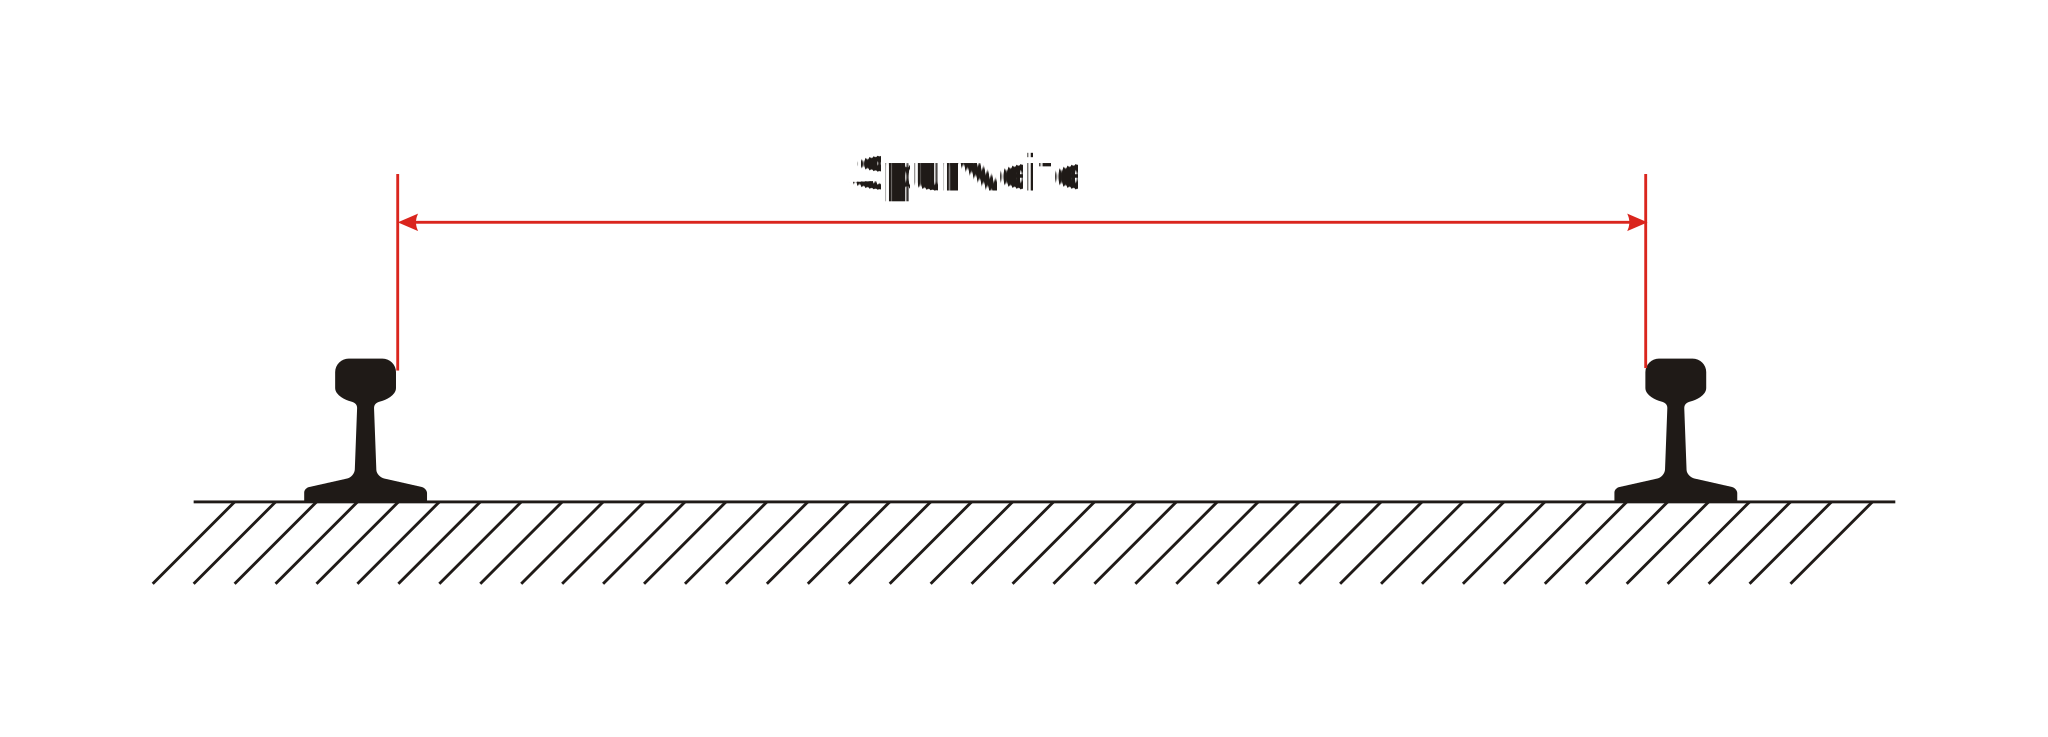
\includegraphics[width=0.8\textwidth]{spurweite}
  \caption{Spurweite Normalspur}
\end{figure}
\noindent
\textbf{Schienenkopf:}
\\

\noindent
Der Schienenkopf beschreibt den oberen Teil der Schiene, welcher für die vorliegende Arbeit besonders von Interesse ist, da dieser die Breite der Schienenmarkierungen darstellt. Das gängige Hauptbahn-Profil ist das S54, welches folgende Maße besitzt:
\\


\noindent
\begin{tabular}[h]{c|c|c|c}
Höhe in mm & Kopf in mm & Steg in mm & Fuß in mm\\
\hline
159 & 67 & 16 & 125 \\
\end{tabular}
\begin{figure}[H]
  \includegraphics[width=0.5\textwidth]{schienenkopf}
  \caption{Schiene S54}
\end{figure}
\noindent
Die Beiden für die Umsetzung des Projektes relevanten Maße sind demnach:
\begin{itemize}
	\item Spurweite: 1435mm
	\item Schienenkopf: 67mm
\end{itemize}

\subsection{Die projektive Ebene}
\label{sec:Die projektive Ebene}

\begin{figure}[H]
  \includegraphics[width=0.8\textwidth]{projektive}
  \caption{Kamera- und Bildkoordinaten}
\end{figure}

\noindent
Die projektive Ebene findet ihren Ursprung in der Malerei der italienischen
Renaissance. Dort versuchte man die Realität, insbesondere die Architektur, korrekt
in Gemälden widerzuspiegeln. Dabei ging es vor allem um projektive Effekte im
unendlichen, wie der Schnitt zweier parallel verlaufender Geraden im imaginären
Fluchtpunkt unter projektiver Abbildung auf eine Ebene.
Die Grundlage projektiver Räume ist durch homogene Koordinaten gegeben, deren
Haupteigenschaft die Invarianz (Unveränderlichkeit) gegenüber Skalierungen ist.
Diese werden durch (n+1)-dimensionale Vektoren beschrieben. Die projektiven
Punkte eines Raumes können sich als Strahlen vorgestellt werden, welche durch
den Ursprung eines 3D-Koordinatensystems verlaufen. Alle auf dem Strahl
befindlichen Punkte sind mit einer Multiplikation eines geeigneten Skalierungsfaktors
ineinander überführbar und somit äquivalent. Dabei existieren für parallel zur jeweils
gewählten Ebene verlaufende Strahlen keine Repräsentanten. Im Sonderfall der
parallel zur x-y-Ebene gelegenen Ebene E : z = 1 ergeben sich alle Repräsentanten
aus den geschnittenen Strahlen durch Skalierung der dritten Vektorkomponenten auf
1.
\\
Diese Arbeit liegt dem Modell der Lochkamera zugrunde, wobei das
Projektionszentrum der Kamera im Ursprung eines 3D-Kamerakoordinatensystems
liegt (siehe Abbildung 18). Die optische Achse fällt mit der z-Achse des
Koordinatensystems zusammen. Im Abstand der Bildweite( focal length) f \textgreater 0 vom
optischen zentrum befindet sich die Bildebene, auf die die 3D-Welt zweidimensional
abgebildet wird (z = 1). Die Bildebene ist dabei stets parallel zur x-y-Ebene des
3D-Koordinatensystems. Der Hauptpunkt an dem die optische Achse die Bildebene
durchstößt, liegt demnach an Position (px,py,1) auf der Ebene. Die Projektion eines
beliebigen 3D-Punktes(Objekt) des Kamerakoordinatensystems auf die Bildebene
ergibt sich in diesem Modell als Schnittpunkt des Richtungsstrahls vom optischen
Kamerazentrum zum Punkt der Kamerakoordinaten(x,y,z) mit der Bildebene. Dabei
ist noch unberücksichtigt geblieben, dass die beiden Koordinatenachsen der
Bildebene in der Regel jeweils unterschiedlich und darüber hinaus unabhängig vom
3D-Koordinatensystem der Kamera skaliert sind. Um die Bildkoordinaten in
Pixelkoordinaten korrekt umrechnen zu können, müssen somit bei der Abbildung in
x- und y-Richtung jeweils spezifische Skalierungsfaktoren berücksichtigt werden.
Durch das Wissen um die Kameraparamter (Brennweite, focal lenght) der
entsprechenden Kameramatrix und der Kameraposition(Translations- und
Rotationsmatrix) können die Weltkoordinaten (entsprechen Größen der realen Welt)
in Bildkoordinaten (Pixel) umgerechnet werden. Dazu wird hintereinander eine
Transformation von Welt → Kamera und Kamera → Bild durchgeführt.
\begin{lstlisting}
	FORMEL HIER
\end{lstlisting}
Das bedeutet, die Bildkoordinaten pimg entsprechen einer Multiplikation der
Kameramatrix K, mit der Rotationsmatrix R|t und den Weltkoordinaten pworld.Bei den Weltkoordinaten handelt es sich um 3-dimensionale Datenpunkte, welche eine x-, y- und z-Achse besitzen. Es können im Umkehrschluss auch
Bild- zu Weltkoordinaten problemlos umgerechnet werden.

\subsection{Berechnung der Messlinie}
\label{sec:Berechnung der Messlinie}

\noindent
Die Messlinie wird im vorliegenden Tool dazu verwendet, die Mittelpunkte der Schiene genau abschätzen zu können und entsprechend genau die Punkte zu setzen. Der exakte Abstand zwischen den beiden Endpunkten der Messlinie wird berechnet,
indem der Mittelpunkt (x-y-Koordinaten) des Mauszeigers an der jeweiligen Position
genommen und durch Matrixmulitplikation in Weltkoordinaten umgerechnet wird. Diese Weltkoordinaten sind Punkte, welche durch einen 3-Dimensionalen Datenpunkt beschrieben werden. In Weltkoordinaten verändert sich die Breite der Schiene und somit der Messlinie nicht, weshalb der Mausmittelpunkt um 1435mm/2\footnote{Länge der Spurweite} auf der x-Achse nach links und rechts verschoben werden können. Danach werden diese Punkte wieder in
Bildkoordinaten umgerechnet, wodurch wir wieder die perspektivische Sicht erhalten.
In allen Berechnungen wird angenommen, dass wir geradeaus schauen und nichts
im Wege ist. Damit sind die Dimensionen nicht mehr variabel und eine Umrechnung
ist möglich.



\subsection{Der Catmull-Rom Spline}

\noindent
Ein zentripetaler Catmull-Rom Spline ist eine stückweise definierte kubische polynomiale Funktion mit mindestens vier Punkten. Nach dem
Setzen des vierten Punktes werden Punkte 1 und 4 als Stützpunkte herangezogen
und zwischen Punkt 2 und 3 eine interpolierte Kurve gezeichnet. Eine Teilkurve zwischen einzelnen Punkten des Splines hört da auf, wo die nächste beginnt. Die beiden Tangenten der jeweiligen Segmentgrenzen stimmen in ihrer Richtung überein, wodurch sich ein weicher Übergang von Segment zu Segment ergibt. Das bedeutet, dass die Tangenten aneinandergrenzender Segmente in ihrem gemeinsamen Punkt gleich sind. Die so interpolierte Kurve besteht dann aus stückweise differenzierbaren Segmenten und ist stetig differenzierbar. 
Möchten wir einen Spline durch k Punkte ziehen, dann brauchen wir insgesamt k+2 Stützpunkte. Aufgrund dieser Eigenschaft kann der Verlauf einer Schiene durch das Setzen von Mittelpunkten exakt abbgebildet werden. Die Verwendung eines Catmull-Rom Splines entstand aus der Vorüberlegung, dass die Verbindungen zwischen Punkten auf der Schiene nur gerade Linien darstellen und somit ein genauer Verlauf einer Kurve sehr viele Punkte vorausgesetzt hätte. Durch die Verwendung des Catmull-Rom Splines können diese Punkte deutlich reduziert werden. Problematisch ist hier, dass der Spline erst ab dem zweiten und lediglich bis zum vorletzten Punkt gezeichnet wird, wodurch Teile der Schiene ausgelassen werden.

\begin{figure}[H]
  \includegraphics[width=0.8\textwidth]{cat}
  \caption{Catmull-Rom Spline}
\end{figure}


\subsection{Analyse des Annotation Tool's von Herrn Mario Hoffmann}
\label{sec:Analyse des Annotation Tool's von Herrn Mario Hoffmann}

Das vorliegende "Annotation Tool" von Herrn Mario Hoffmann wurde im Rahmen des Projekts SE Perception zum qualitativen Labeln von Mittelpunkten einer Schiene erstellt. Dazu sollten immer gleich viele Mittelpunkte in einem festen Abstand auf einem Bild markiert werden. Diese Daten wurden dafür verwendet ein Neuronales Netzwerk auf die Erkennung von Mittelpunkten zu trainieren. Es existierend zu diversen Bildern Mittelpunkt-Datein, welche später dazu genutzt werden sollen Schienenmarkierungen daraus generieren zu können. Die Funktionen werden hier und im weiteren Verlauf konzeptionell dargstellt und entsprechen keiner bestimmten Programmiersprache. Diese Abstraktion soll der Verständlichkeit dienen.

\subsubsection{Informelle Beschreibung und komplxitätsanalyse}
\label{Informelle Beschreibung und komplxitätsanalyse}

\textbf{Installation auf einem Linux-basierenden Betriebssystem:} 
\begin{itemize}
	\item OpenCV, Version, bevorzugt 3.4.7 und gcc Toolchain installieren
	\item Cmake installieren
	\item git clonen
	\item In das Verzeichnis wechseln: cd Videoplayer
	\item Build directory erstellen und in Dieses wechseln: mkdir -p build cd build
	\item CMake konfigurieren und Anwendung kompilieren: cmake .. make
\end{itemize}
\noindent
Das Programm "Annotation Tool" bietet dem Nutzer die Möglichkeit einen Ordner von Bildern und eine Kamera-Matrix einzulesen und dann realitätsgetreu durch Abbildung der projektiven Ebene Mittelpunkte von Schienen markieren zu können. Das Programm wurde in C++ unter Verwendung der OpenCV Bibliothek realisiert.  Der grobe Ablauf kann folgendermaßen dargestellt werden:

\begin{enumerate}
	\item der User startet das Programm über den Terminal (Linux) mit folgendem Befehl: ./videoplayer - -label -yaml="Pfad zur Kamera-Matrix" "Pfad zu den Bildern"
	\item das Programm öffnet sich und zeigt das Bild samt Hilfslinie
	\item der User wählt zwischen "x", "y" und "c" für Mittelschiene, linke Schiene oder rechte Schiene
	\item das Programm zeigt die Hilfslinie in der korrespondierenden Farbe an
	\item der User bewegt den Mauszeiger über die Schiene und versucht unter Verwendung der Hilfslinie die Mitte der Schiene abzuschätzen
	\item der User setzt mit "d" entlang der Equidistant (gleicher Abstand) Linien die Mittelpunkte der Schiene
	\item das Programm speichert die Mittelpunkte in einem Vektor
	\item der User speichert mit "s" die Mittelpunkte in einer yaml-Datei
	\item das Programm schreibt eine Datei mit den Mittelpunkten im yaml-Format
	\item der User wechselt mit "n" zum nächsten Bild
	\item das Programm wechselt auf das nächste Bild
	\item der User beendet mit "q" das Programm
	\item das Programm beendet sich
\end{enumerate}
\noindent
Diese Funktionalitäten wurden durch verschiedene Bibliotheken realisiert, welche vorher installiert werden müssen. 
Verwendete Bibliotheken:

\begin{itemize}
	\item OpenCV, Version 3.4.7 Algorithmen für die Bildverarbeitung und Computer Vision
	\item nlohnmann JSON für Modern C++ für die Mittelpunkt-Datein
\end{itemize}
\noindent
Neben diesen Bibliotheken wurden noch weitere Headerdatein eingebunden, um Funktionalitäten aus dem Videoplayer und die Berechnungen von Welt- und Pixelkoordinaten nutzen zu können:

\begin{itemize}
	\item "Videoplayer.h"
	\item "Camera.h"
\end{itemize}

\noindent
Das Programm setzt sich im Ausgangzustand aus einer Header-File, in der Datentypen und Funktionen deklariert werden und einer .cpp-Datei, welche die Implementierung der Logik beinhaltet, zusammen. Es besteht aus 425 Zeilen Code und eine Fehlerbehandlung ist nur rudimentär vorhanden. Zum speichern der Punkte in Vektoren wird ein Struct verwendet, welches den Namen "LabelImage" trägt. Im weiteren Verlauf dieser Arbeit wird ein solcher Struct als "LabelImage" bezeichnet. Das Programm liest aus der Command-Zeile per Commandline-Parser die Pfade zu den Bildern und der Kamera-Matrix. Beim Ausführen wird zunächst die Bedienungsanleitung angezeigt. Danach werden die angegebenen Bilder eingelesen und zu jedem Bild ein "LabelImage"-Struct erstellt. Nach dem Einlesen startet das Labeltool und liest die Kamera-Matrix und die eventuell vorhandene yaml-Datein für die Mittelpunkte ein. Den Hauptteil des Programms stellt eine while-Schleife dar, welche mit jedem Durchlauf das eingelesene Bild in ein neues Mat-Objekt kopiert, damit die Hilfslinie immer auf einem neuen Bild gezeichnet wird und somit der Effekt entsteht, dass es sich dabei um eine dynamisch-bewegbare Linie handelt. Weiterhin wird in dieser Schleife der User-Input verwertet und die Funktionen zum Speichern der Punkte ausgeführt. Das Struct "LabelImage" enthält folgende Attribute:
\begin{itemize}
	\item string name
	\item string basename
	\item vector\textless Point\textgreater leftPts
	\item vector\textless Point\textgreater rightPts
	\item vector\textless Point\textgreater centerPts
\end{itemize}
\noindent
Die Vektoren wurden mit dem OpenCV Datentypen Point deklariert. Dieser Datentyp stellt eine Template Klasse für 2D-Punkte mit x- und y-Koordinate dar. Somit repräsentieren diese Punkte die Mittelpunkte der linken, rechten und Mittelschiene im Bild in Pixelkoordinaten.
\\

\noindent
Das Programm kannfolgendermaßen aufgegliedert werden:
\begin{itemize}
	\item Filehandling - Einlesen der Bilder, yaml-Datein und Kamera-Matrix
	\item Inputhandling - Verwertung von Usereingaben
	\item Punkte speichern und löschen - Speichern der Punkte in Vektoren des Structs "LabelImage"
	\item Hilfslinie anzeigen - zeichnen der Hilfslinie am Punkt der Maus
	\item Berechnung der Equidistant-Linien - exakte Abstände zwischen Horizont und erstem Punkt auf der z-Achse
	\item Output generieren - schreiben der yaml-Datei mit OpenCV Filestorage
\end{itemize}

\noindent
\\
\textbf{Filehandling:}
\noindent
Das Filehandling übernehmen die Funktionen:
\begin{itemize}
	\item void readImageList(path,  lblList)
	\item readJson(lblImages)
	\item Camera(yamlFileName) aus dem "Camera.h"-Include
\end{itemize}

\noindent
Die Funktion readImageList(path,  lblList) bekommt als Input einen Pfad und einen Vektor vom Typ "LabelImage" auf dem die "LabelImages" gespeichert werden. Danach wird mit einem Directory-Iterator über die Bilder im Pfad iteriert. Für jedes Bild wird ein Struct "labelImage" erstellt, das "LabelImage" nach dem jeweiligen Bild benannt und danach auf dem Vektor "lblList" gespeichert. Die readJson(lblList) bekommt als Input die Liste der gespeicherten "LabelImages" und sucht in dem gleichen Directory nach einer Datei, welche den selben Namen jedoch als Dateiendung ".yaml" trägt. Danach werden mit der OpenCV Filestorage Klasse die Punkte aus der yaml-Datei in den Vektoren der "LabelImages" gespeichert. Die Klasse Camera(yamlFileName) wird mit dem Pfad der Kamera-Matrix aufgerufgen und lädt diese Kamera-Matrix durch den Constructor unter Verwendung der OpenCV Filestorage Klasse.


\noindent
\\
\textbf{Inputhandling:}
\noindent
In der While-Schleife erwartet die OpenCV-Funktion waitkey() die Eingabe eines Buchstaben durch den Benutzer. Danach wird diese Eingabe in einem Switch-Case ausgewertet und entsprechende Funktionen der einzelnen Cases ausgeführt. Dieses einfache Vorgehen war möglich, da das Programm nur wenige Eingabemöglichkeiten aufweist. Dieses Struktur wird in der späteren Eigenprogrammierung übernommen und deshalb nicht weiter erläutert.

\noindent
\\
\textbf{Punkte speichern und löschen:}
\noindent
Diese Funktionalitäten wurden durch folgende Funktionen realisiert:
\begin{itemize}
	\item void savePoint(Point , LabelImg, equidistantY)
	\item void removeClosestPoint(LabelImg)
\end{itemize}

\noindent
Zum Speichern eines Punktes wird der savePoint(Point , LabelImg, equidistantY)-Funktion die momentane Mausposition als OpenCV Datentyp Point, das jeweilige "LabelImage" und die Equidistant-Punkte übergeben. Beim Speichern wird abgefragt, wie weit der Cursor sich von den Equidistant-Linien entfernt befindet und sollten dies weniger als 10 Pixel sein, dann wird der Punkt automatisch auf dieser Linie gesetzt und auf dem Vektor Equidistantpoints des "LabelImage" gespeichert. Danach wird mit einem Switch-Case überprüft, welche Schiene angewählt ist und entsprechend der Punkt auf dem jeweiligen Vektor gespeichert. Gelöscht werden die Punkte durch die Abfrage in einem Switch-Case, welche Schiene angewählt ist. Danach wird ein Pointer auf den Adressspeicher des jeweiligen Vektors initialisiert. Sollte der momentane Mauspunkt näher als ein bestimmter Schwellenwert (hier 200 Pixel) sein, dann wird dieser Adressspeicher freigegeben und der Punkt dadurch gelöscht.

\noindent
\\
\textbf{Hilfslinie anzeigen:}
\noindent
Diese Funktionalitäten wurden durch folgende Funktionen realisiert:
\begin{itemize}
	\item void drawArTrack(img, LabelImg)
\end{itemize}

\noindent
In dieser Funktion werden die momentanen Korrdinaten des Mauszeigers genommen und von Pixel- in Weltkoordinaten umgerechnet(Beschrieben in Kapitel: Grundlagenforschung). Dieser Punkt wird dann um jeweils (-1435/2)\footnote{1435mm ist der exakt genormte Abstand zwischen der linken und rechten Schiene} nach links und (1435/2) nach rechts verschoben. Dort werden diese Punkte wieder in Pixelkoordinaten umgerechnet, sodass durch die Open CV circle() und line() Funktionen die Hilfslinie auf dem Bild gezeichnet werden können. Da in der while-Schleife bei jedem Durchlauf auf einem neuen Bild gezeichnet wird, entsteht der Effekt einer sich frei bewegenden Linie.
\\

\noindent
\textbf{Berechnung der Equidistant-Linien :}
\\

\noindent
Diese Funktionalitäten wurden durch folgende Funktionen realisiert:
\begin{itemize}
	\item void getEquidinstantY(image)
\end{itemize}

\noindent
Diese Funktion errechnet anhand eines gegebenen Horizonts und dem ersten sich im Bild befindlichen Punkt auf der z-Achse die Equidistant-Linien. Dafür wird zunächst eine z-Achse definiert, welche den ersten im Bild sichtbaren Punkt z auf der z-Achse in Weltkoordinaten umgerechnet. Danach werden mit einer Forschleife,  einem in Weltkoordinaten festgelgten Horizonts und einer festen Anzahl an Linien die Punkte auf der z-Achse im gleichen Abstand errechnet.
\begin{lstlisting}
for (int i = 0; i <= numLines; ++i ){
        y =  horizontPoint   n - (i * ((horizontPoint- z)/numLines));
        Point3d HWorld = Point3d(0, 0, y);
        horizonLine = kam.world2pixel(HWorld);
        eq.push_back(horizonLine.y);
}
\end{lstlisting}

\noindent
\\
\textbf{Output generieren:}
\noindent
Diese Funktionalitäten wurden durch folgende Funktionen realisiert:
\begin{itemize}
	\item void writeJson(lblList)
\end{itemize}
\noindent
\\
Diese Funktion bekommt die Liste mit den "LabelImages" und iteriert über diese mit einer Forschleife. Danach wird für jedes "LabelImage" ein Open CV Filestorage geöffnet und die Punkte in einem entsprechenden Format in die Datei geschrieben.

\subsubsection{Anforderungsdiagramme "AnnotationTool"}
\label{sec:Anforderungsdiagramme "AnnotationTool"}

Für das Programm "AnnotationTool" lässt sich folgender Anwendungsfall identifizieren:
\\

\noindent
\textbf{S1 : Mittelpunkt Generierung:} 
	
\noindent
A)
\begin{itemize}
	\item Der Nutzer liest das Schienenbild
	\item Der User erstellt, löscht oder bearbeitet die Mittelpunkte
	\item Der User speichert die Punkte in einer Datei
	\item Der User wechselt zum nächsten/vorherigen Bild
\end{itemize}

\begin{figure}[H]
  \includegraphics[width=0.8\textwidth]{newusecaseannotation}
  \caption{Anwendungsfall A AnmnotationTool}
\end{figure}

B)
\begin{itemize}
	\item Der Nutzer liest das Schienenbild und existierende Mittelpunkte aus einer Datei
	\item Der User erstellt, löscht oder bearbeitet die Mittelpunkte
	\item Der User speichert die Punkte in einer Datei
	\item Der User wechselt zum nächsten/vorherigen Bild
\end{itemize}

\begin{figure}[H]
  \includegraphics[width=0.8\textwidth]{newusecaseannotation2}
  \caption{Anwendungsfall B AnmnotationTool}
\end{figure}

\section{Anforderungen an das Programm }
\label{sec:Anforderungen an das Programmn}
\subsection{Anforderungen aus Kundensicht}
\label{sec:Anforderungen aus Kundensicht}

\noindent
Bei der Produktentwicklung und Prozessoptimierung ist eine Anforderung ein einzelnes dokumentiertes physisches oder funktionales Bedürfnis, das ein bestimmtes Design, Produkt oder Verfahren erfüllen soll. Im Rahmen des Entwicklungsprozesses wird eine geeignete Methode gefordert, um diesen exakt beschreiben zu können. Dabei fiel die Wahl auf die Unified Modeling Language (UML) , da diese in der Lage ist nahezu jedes reale Weltbild digital zu erfassen und mittels eines Modells unabhängig von Programmiersprachen zu beschreiben. Die aufgestellten Anforderungsdiagramme wurden in Englisch geschrieben, da sie im Rahmen des Projektes und nicht in direkter Abhängigkeit zu dieser Arbeit entstanden sind. 
\\

\noindent
Zur Realisierung des Labeltoolls wurden folgende Szenarios  aufgestellt:
\\

\noindent
\textbf{S1 : Centerpointlabeling:} 
	
\noindent
A)
\begin{itemize}
	\item Der Nutzer liest das Schienenbild
	\item Der User erstellt, löscht oder bearbeitet die Mittelpunkt-Labels
	\item Der User speichert die Punkte in einer Datei
\end{itemize}

\begin{figure}[H]
  \includegraphics[width=0.6\textwidth]{newusecase1new}
  \caption{Use Case Szenario 1}
\end{figure}

B)
\begin{itemize}
	\item Der Nutzer liest das Schienenbild und existierende Mittelpunkte aus einer Datei
	\item Der User erstellt, löscht oder bearbeitet die Mittelpunktt-Labels
	\item Der User speichert die Punkte in einer Datei
\end{itemize}

\begin{figure}[H]
  \includegraphics[width=0.6\textwidth]{newusecases2}
  \caption{Use Case Szenario 2}
\end{figure}

\noindent
\textbf{S2 : Segmentationslabel Generierung:} 
	
\noindent
A)
\begin{itemize}
	\item Der Nutzer liest das Schienenbild und existierende Mittelpunkte aus einer Datei
	\item Das Programm überprüft, ob die notwendigen Informationen vorhanden sind
	\item Das Programm generiert die Segmentierungsinformationen
	\item Der User speichert die Segmentierungsinformationen
\end{itemize}

\begin{figure}[H]
  \includegraphics[width=0.7\textwidth]{newusescases3}
  \caption{Use Case Szenario 3}
\end{figure}

\noindent
\textbf{S3 : Manuelle Segmentierungslabel Augmentation :} 
	
\noindent
A)
\begin{itemize}
	\item Der Nutzer liest das Schienenbild und existierende Vektorpunkt-Datei der Labels
	\item Der Nutzer ändert vorhandene Labels oder erstellte neue Labels für autogenerierte Labels
	\item Der Nutzer fügt Labelregionen hinzu, welche nicht durch Segmentierungslabelgenerierung berücksichtig werden
	\item Der User speichert die Segmentierungsinformationen
\end{itemize}

\begin{figure}[H]
  \includegraphics[width=0.6\textwidth]{usecase4}
  \caption{Use Case Szenario 4}
\end{figure}


\begin{itemize}
	\item Der Nutzer liest das Schienenbild und existierende Vektorpunkt-Datei der Labels
	\item Der Nutzer ändert vorhandene Labels oder erstellte neue Labels für autogenerierte Labels
	\item Der Nutzer fügt Labelregionen hinzu, welche nicht durch Segmentierungslabelgeneration berücksichtig werden
	\item Der User speichert die Segmentierungsinformationen
\end{itemize}

\noindent
\textbf{Soll-Anforderungen: } 
\\

\noindent
\underline{LH-Anforderung: Filehandling}
\\
\noindent
LH 1.    Das System soll Bilder einlesen können 
\\
\noindent
LH 1.1   Das System soll Markierungsinformationen zu jedem Bild einlesen können
\\
\noindent
LH 2 Das System soll eingelese Markierungsinformationen darstellen können
\\

\noindent
\underline{LH-Anforderung: Punkte speichern und löschen}
\\
\noindent
LH 3.    Das System soll neue Marikerungen durch Punkte im Bild erstellen können
\\
\noindent
LH 3.1 Das System soll vorhandene Punkte verändern können
\\
\noindent
LH 3.2 Das System soll die Schienen exakt Abbilden können
\\

\noindent
\underline{LH-Anforderung: Output generieren}
\\
\noindent
LH 4    Das System soll prüfen, ob Segmentierungsinformationen vorhanden sind
\\
\noindent
LH 5   Das System soll erstellte Markierungsinformationen in einer Datei speichern
\\
\noindent
LH 6  Das System soll Segmentierungsinformationen generieren
\\

\noindent
\subsection{Abgeleitete Anforderungen}
\label{sec:Abgeleitete Anforderungen}

Durch die Analyse der Anforderungen und des zugrunde liegenden AnnotationTools, können nun Anforderungen für die eigene Software abgeleitet werden.

\subsubsection{S1 : Mittelpunkt Generierung} 
\label{sec:S1 : Mittelpunkt Generierung}

A)
\noindent
Im Vergleich der Anforderungen mit dem in Kapitel XX beschriebenen AnnotationTool wird deutlich, dass das Grundgerüst für diesen Anwendungsfall gegeben ist, da sowohl das Einlesen der Kamera-Matrix, yaml-Datein und der Bilder vorhanden ist. Aufbauend darauf muss die Software hier um die Berechnung der Schienenlabel erweitert werden, sodass die Mittelpunkte dazu genutzt werden können, daraus die Schienenlabel zu erstellen.  Da die Software von Herrn Hoffmann nur zwischen der Mittelschiene, dem rechten Nachbar und dem linken Nachbar unterscheiden kann, muss hier zusätzlich implementiert werden, dass beliebig viele Nachbarn und deren Markierungen erstellt werden können. Da Punkte nun nicht mehr in der Mitte der Schiene, sondern auf der Mitte der Schienenköpfe gesetzt werden, müssen die Messlinie und die Funktion zum Speichern der Punkte verändert werden. Zudem muss die Funktion zum Erstellen der yaml-Datei angepasst werden, sodass die Schienenkopfmittelpunkte gespeichert werden können. 
\\

\noindent
B)
\noindent
Im Anforderungfall B wird geforderet, dass die Mittelpunkte, welche für Benchmarks der Algorithmen zur Schienenerkennung genutzt werden sollen, der Schiene aus einer Datei gelesen, entsprechend verändert und gespeichert werden sollen. Da das Einlesen von Mittelpunkten schon vorhanden ist, muss in diesem Fall keine Veränderung vorgenommen werden. Da weitere Punkte auf den Schienen hinzukommen, muss zusätzlich eine weitere Funktion geschrieben werden, welche die neue Datein mit den Punkten auf die Schienen schreiben und einlesen kann. Die alte Funktion des Einlesens der Mittelpunkte soll aber weiterhin gegeben sein, sodass auch schon existierende yaml-Datein dazu genutzt werden können daraus Schienenlabel zu erstellen. Dies spart Zeit und Ressourcen.
\\

\noindent
\textbf{Abgeleitete Anforderungen Musskriterien:}

\begin{itemize}
	\item Berechnung der Label für die Schienen aus den Mittelpunkten
	\item beliebig viele Label der Nachbarschienen
	\item Speichern der Schienenkopfmittelpunkte
	\item Lesen des neuen Datei-Formats 
	\item Schreiben des neuen Datei-Formats
\end{itemize}
\textbf{Abgeleitete Anforderungen Wunschkriterien:}
\begin{itemize}
	\item Einlesen mehrerer Datei-Formate 
\end{itemize}
\textbf{Abgrenzungskriterien:}

\begin{itemize}
	\item Das Programm markiert keine anderen Klassen als Schienen 
	\item Das Programm verwendet nur ein konkretes Dateiformat
\end{itemize}

\noindent
\subsubsection{S2 : Segmentationslabel Generierung} 
\label{sec:S2 : Segmentationslabel Generierung}
A)
\noindent
In diesem Anwendungsfall sollen Segmentierungsinformationen gespeichert werden, damit diese sowohl für das Training des neuronalen Netzwerks, als auch in einem weiteren Anwendungsfall von einem Drittanbieter-Programm verarbeitet und erweitert werden können. Dabei handelte es sich um folgende Daten:
\begin{itemize}
	\item Pixelmasken der Schienenlabel
	\item Ground Truth des Schienenlabels
	\item Vektorpunkte der Label für Drittanbieter
\end{itemize}
\noindent
Das vorliegende AnnotationTool bietet keine dieser Funktionalitäten, weshalb diese implementiert werden müssen. Dazu muss gesichert sein, dass das Programm wie in S1 beschrieben, entsprechende Informationen in Form von Punkten in einem Vektor generiert. Das Programm wandelt die existierende Schienenlabel erst in eine Pixelmaske und dann in Ground Truth Daten um. 
Weiterhin müssen ein Drittanbieter-Programm und das Input-Format ausgewählt werden. Es muss eine Funktion geschrieben werden, welche diese Vektorpunkte in das ausgewählte Format konvertiert, damit diese vom Drittanbieter verstanden werden können. Eine Abfrage, ob alle notwendigen Informationen gegeben sind soll auch implementiert werden. Es wäre wünschenswert, dass das Programm die Vektorpunkten in verschiedenen gängigen Formaten ausgeben könnte, damit man nicht auf einen bestimmten Drittanbieter angewiesen ist, sollte ein bestimmtes Format nur von diesem unterstützt werden.
\\

\noindent
\textbf{Abgeleitete Anforderungen Musskriterien:}

\begin{itemize}
	\item Abfrage der notwendigen Informationen
	\item Erstellen einer Pixelmaske aus den Schienenlabels
	\item Erstellen von Ground Truth Daten aus der Pixelmaske
	\item Erstellen einer Datei mit den Vektorpunkten
\end{itemize}
\textbf{Abgeleitete Anforderungen Wunschkriterien:}

\begin{itemize}
	\item Verschiedene Formate für Vektorpunkt-Datei
\end{itemize}
\textbf{Abgrenzungskriterien:}

\begin{itemize}
	\item Das Programm gibt die Vektorpunkte nur in einem bestimmten Format aus
	\item Die Klassen der Ground Truth Daten basieren auf einer Erweiterung des "Railsem19" Datensatzes
\end{itemize}

\subsubsection{S3 : Manuelle Segemtierungslabel Augmentation} 
\label{sec:S2 : Segmentationslabel Generierung}
A)
\noindent
Dieser Anwendungsfall beschreibt die Nutzung eines Drittanbieter-Tools, welches die vom LabelTool generierte Vektorpunkt-Datein einliest und die entsprechenden Label korrekt anzeigt. Danach werden diese Label durch das Drittanbieter-Tool erweitert und die Informationen gespeichert. Als Kritierien können hier lediglich die Korrektheit der Vektorpunkt-Datein abgeleitet werden. Wünschenswert wäre es, wenn das Programm ausgewählte Vektorpunkte-Datein von Drittanbietern lesen und erweitern könnte. So wäre man unabhänging von der Prozess-Reihenfolge, wenn mehr Label als nur Schienen erstellt werden sollen.
\\

\noindent
\textbf{Abgeleitete Anforderungen Musskriterien:}

\begin{itemize}
	\item Korrektheit der Labelinformationen
\end{itemize}
\textbf{Abgeleitete Anforderungen Wunschkriterien:}

\begin{itemize}
	\item Lesen von Vektorlabeldatein von Drittanbietern
\end{itemize}
\textbf{Abgrenzungskriterien:}

\begin{itemize}
	\item Es wird sich auf einen Drittanbieter zum Einlesen der Vektorpunkt-Datein beschränkt
\end{itemize}
\noindent
\textbf{Pflicht-Anforderungen: } 
\\

\noindent
In den Pflichtanforderungen werden Kriterien beschrieben, welche zur Umsetzung des Projektes nötig sind
\\ 

\noindent
\underline{PH-Anforderung: Filehandling}
\\
\noindent
PH 1    Das System muss die Kamera-Matrix einlesen können
\\
\noindent
PH 2  Das System muss Bilder einzeln, oder aus einem Ordner einlesen können
\\
\noindent
PH 2.1 Das System muss existierende Markierungsinformationen zu den Bildern automatisch einlesen können
\\
\noindent
PH 2.2 Das System muss Mittelpunktinformationen einlesen können
\\
\noindent
PH 2.3 Das System muss Schienenpunktinformationen einlesen können
\\
\noindent
PH 3  Das System muss aus eingelesenen Informationen Schienenmarkierungen generieren können
\\

\noindent
\underline{PH-Anforderung: Punkte speichern und löschen}
\\
\noindent
PH 4   Das System muss beliebig viele Schienenmarkierungen generieren können
\\
\noindent
PH 4.1 Das System muss zwischen rechtem und linkem Nachbar unterscheiden können
\\
\noindent
PH 5 Das System muss zwischen den jeweiligen Schienenmarkierungen wechseln können
\\
\noindent
PH 5.1 Das System muss die angewählten Schienenmarkierungen verändern können
\\
\noindent
PH 5.2 Das System muss die Länge der Messlinie anpassen können
\\

\noindent
\underline{PH-Anforderung: Output generieren}
\\
\noindent
LH 6  Das System muss prüfen, ob Segmentierungsinformationen vorhanden sind
\\
\noindent
PH 7 Das System muss vorhandene Markierungen von Schienen- und Mittelpunkten wiedereinlesbar in einer Datei speichern
\\
\noindent
PH 8   Das System muss Segmentierungsinformationen generieren können
\\
\noindent
PH 8.1  Das System muss eine Pixelmaske generieren können
\\
\noindent
PH 8.2 Das System muss aus der Pixelmaske Ground Truth Daten erstellen können
\\
\noindent
PH 8.3 Das System muss eine Vektorpolygon-Datei zur Verwendung bei Drittanbietern generieren können
\\

\noindent
\textbf{Abgedeckt durch das AnnotationTool von Herrn Hoffmann:}
\\


\noindent
\begin{tabular}[h]{c|c|c}
Kategorie & Anforderung LH & Anfoderung PH \\
\hline
Filehandling & LH 1 & PH 1 \\
Filehandling & LH 1 & PH 2 \\
Filehandling & LH 1.1 & PH 2.1 \\
Filehandling & LH 1.1 & PH 2.2 \\
\end{tabular}
\\
\\

\noindent
\textbf{Notwendige Implementierungen:}
\\


\noindent
\begin{tabular}[h]{c|c|c}
Kategorie & Anforderung LH & Anfoderung PH \\
\hline
Filehandling & LH 1.1 & PH 2.3\\
Filehandling & LH 2 & PH 3\\
Punkte speichern und löschen & LH 3 & PH 4 \\
Punkte speichern und löschen & LH 3 & PH 4.1 \\
Punkte speichern und löschen & LH 3 & PH 5 \\
Punkte speichern und löschen & LH 3.1 & PH 5.1 \\
Punkte speichern und löschen & LH 3.2 & PH 5.2 \\
Output generieren & LH 4 & PH 6 \\
Output generieren & LH 5 & PH 7 \\
Output generieren & LH 6 & PH 8 \\
Output generieren & LH 6 & PH 8.1 \\
Output generieren & LH 6 & PH 8.2 \\
Output generieren & LH 6 & PH 8.3 \\


\end{tabular}

\newpage
\section{Konzeptioneller Entwurf }
\label{sec:Konzeptioneller Entwurf}

Die Idee hinter der Eigenprogrammierung versucht die vorher erklärten Sachverhalte in einen Kontext zu bringen. 

\subsection{Erweiterung der Grundidee}
\label{sec:Erweiterung der Grundidee}

\noindent
Die Grundidee wurde aufgegriffen und folgendermaßen erweitert:
\\
Die Idee des LabelTools beschreibt die semi autogenerierte Markierung von Schienen anhand der Möglichkeit, dass Pixel- in Weltkoordinaten umgerechnet und dann realitätsnah im Bild verschobenen werden können. Durch Verwendung der Messlinie und unter Berücksichtigung der Erarbeiteten Schienenmaße, können Punkte auf der Mitte des Schienenkopfes exakt bestimmt werden. Da Schienen jedoch Kurven aufweisen und man in diesen viele Punkte setzen müsste, damit eine Markierung korrekt auf die Schiene abbildet, wurde ein Catmull-Rom Spline verwendet. Die Funktion wird durch die entsprechenden Pixelkoordinaten der Schienenmittelpunkte auf dem Bild gezeichnet. Die beliebig vielen Schritte während der Interpolation können dazu genutzt werden, die jeweiligen Pixelkoordinatenpunkte auf dem Spline in Weltkoordinaten umzurechnen, dann um die Maße eines halben Schienenkopfes nach links und rechts zu verschieben und dann zurückgerechnet als Pixelkoordinate gespeichert zu werden. Somit repräsentieren die gespeicherten Punkte den linken und rechten Rand der Schiene mit einer zentripetalen polynominalen Interpolation dritten  Grades durch die Mittelpunkte auf der Schiene. Um Markierungen aus den Mittelpunkten der Schiene generieren zu können, müssen diese nur um die Hälfte der Spurweite addiert mit einer Schienenkopfbreite nach links und rechts in Weltkoordinaten verschoben werden. Diese Punkte Markieren wieder die Mitte der Schiene, welche für den Catmull-Rom Spline genutzt werden. In diesem Ansatz werden also Punkte auf der Mitte des Schienenkopfes gesetzt und nicht wie gewohnt in der Mitte der Schiene.

\begin{figure}[H]
  \includegraphics[width=0.8\textwidth]{schienepunkte}
  \caption{Berechnung der Schienenränder}
\end{figure}


\subsection{Konzept}
\label{sec:Konzept}

Der konzeptionelle Entwurf soll mit dem Anwendungsfall-Diagramm für die Software zum semiautomatischen Labeln von Schienen begonnen werden. Danach erfolgt eine Übersicht über das Flussdiagramm und die Implementierungen. Abschließend werden die Ergebnisse in einer Qualitätsanalyse kritisch betrachtet. Die in den vorangegangenen Kapiteln aufgenommenen Anforderungen und Begrifflichkeiten sollen hier direkt in die Modellbildung mit einbezogen werden. Der schriftlichen Ausarbeitung, welche zur Verständlichkeit in einem hohen Abstraktionslevel gehalten wird, folgen Diagramme, welche die wesentlichen Funktionalitäten der Software modellhaft dokumentieren.

\subsubsection{Anwendungsfall-Diagramm "Labeltool" Grundsystem}
\label{sec:Anwendungsfall-Diagramm "Labeltool" Grundsystem}
An diesem Anwendungsfall ist nur der Aktor "User" beteiligt. Er beschriebt die Kernfunktionalitäten des vorliegenden Systems.

\begin{figure}[H]
  \includegraphics[width=0.8\textwidth]{usecaselabelgrund}
  \caption{Grundsystem LabelTool}
\end{figure}

\noindent
\textbf{Use Case:} Bild labeln
\\ 

\noindent
\textbf{Kurzbeschreibung:} Der User möchte die Schienen in einem Bild markieren, damit diese in maschinenverständliche Daten umgewandelt werden, um ein neuronales Netzwerk damit trainieren zu können. Für Benchmarks und andere Anwendungen sollen neben den Punkten auf den Schienen auch die Mittelpunkt in einer yaml-Datein gespeichert werden. Zuletzt soll eine Datei generiert werden, welche die Polygonpunkte von Labels einem Drittanbieter zur Weiterverarbeitung verständlich macht.
\\ 

\noindent
\textbf{Primärer Aktor:} User
\\ 

\noindent
\textbf{Vorbedingungen:} Die Bilder, welche in das Programm geladen werden sollen, müssen auf dem Computer gespeichert sein. Es muss eine lesbare Kamera-Matrix-Datein vorhanden sein. 
\\ 

\noindent
\textbf{Nachbedingung:} Wenn ein Bild markiert wurde, dann werden die Schienen und das Schienenbett mit eigenen Labels exakt abgebildet. Werden die Segmentierungsinformationen generiert, dann besitzt das konvertierte Bild den Datentyp uint8. Werden die Labels gespeichert, dann wird eine extra Datei erstellt, welche nur die Labels beinhaltet, die in einem anderen Programm neu geladenen und wieder bearbeitet werden können.
\\ 

\noindent
\textbf{Erfolgsszenario:}

\begin{enumerate}
	\item Der User startet das Programm mit den Parametern der Kamera-Matrix und des Bilderordners
	\item Das Programm lädt die Kamera-Matrix und zeigt das erste Bild aus dem Ordner an
	\item Das Programm erstellt ein neues Label "Ego Track" und wählt dieses aus
	\item Der User kalibriert die Messlinie
	\item Das Programm verlängert, verkürzt die Messlinie oder wechselt die Fokusseite
	\item Der User setzt Punkte entlang der Schiene
	\item Das Programm speichert die Punkte in einem Vektor und berechnet damit das Catmull Rom-Polygon
	\item Das Programm zeichnet das Label aus dem Catmull Rom-Polygon-Vektor
	\item Der User erstellt ein neues Label während er seine Maus links oder rechts neben dem "Ego Track" für das jeweilige Label hält
	\item Das Programm erkennt auf welcher Seite ein neues Label erstellt werden soll und erstellt dieses
	\item Der User setzt Punkte entlang der Schiene
	\item Das Programm speichert die Punkte in einem Vektor und berechnet damit das Catmull Rom-Polygon
	\item Das Programm zeichnet das Label aus dem Catmull Rom-Polygon-Vektor
	\item Der User wechselt auf das nächste Bild
	\item Das Programm erstellt die Segmentierungsinformationen und speichert diese in seperaten Ordnern
	\item Das Szenario endet erfolgreich
\end{enumerate}
\textbf{Erweiterungen:}
\\ 
\noindent
(4-15)a. Der User beendet das Programm
\\ 
\noindent
(4-15)a.1 Das Programm beendet sich
\\ 
\noindent
(4-15)a.2 Das Szenario endet erfolglos
\\

\noindent
(1-2)a. Der User gibt eine falsche Kamera-Matrix-Datei an
\\ 
\noindent
(1-2)a.1 Das Programm zeigt an, dass die Kamera-Matrix-Datei nicht gelesen werden konnte
\\ 
\noindent
(1-2)a.2 Das Szenario endet erfolglos
\\ 

\noindent
(1-3)b. Es befinden sich schon yaml-Datein mit Mittelpunkten der Schienen im Bilderordner
\\ 
\noindent
(1-3)b.1  Das Programm erstellt ein neues Label, speichert die Punkte in einem Vektor und berechnet damit das Catmull Rom-Polygon
\\ 
\noindent
(1-3)b.2 Das Programm zeichnet das Label aus dem Catmull Rom-Polygon-Vektor
\\

\noindent
(9-13)a Der User wählt eine andere Schiene aus
\\ 
\noindent
(9-13)a.1 Das Programm selektiert die neu angewählte Schiene
\\

\noindent
(6-13)a. Der User löscht einen Punkt auf der ausgewählten Schiene
\\ 
\noindent
(6-13)a.1 Das Programm entfernt diesen Punkt aus dem Vektor und berechnet das Catmull Rom-Polygon neu
\\ 
\noindent
(6-13)a.2 Das Programm zeichnet das Label aus dem Catmull Rom-Polygon-Vektor
\\ 

\noindent
(6-13)b. Der User löscht ein Label
\\ 
\noindent
(6-13)b.1 Das Programm entfernt das Label 
\\ 

\noindent
(14-15)a Es befinden sich schon Segemtierungsdaten mit der gleichen Bezeichnung in den Ordnern
\\ 
\noindent
(14-15)a.1 Das Programm speichert die Daten nur, wenn der "Saving Modus" aktiv ist

\subsubsection{Anwendungsfall "start"}
\label{sec:Anwendungsfall "start"}

Der Start des Programms beinhaltet folgende Schritte:
\\

\noindent
"load camera matrix"
\begin{itemize}
	\item Der User startet das Programm unter Angabe der Kameramatrix, sollte diese nicht den Vorgaben entsprechen, startet das Programm nicht
\end{itemize}
"load image"
\begin{itemize}
	\item Der User startet das Programm unter Angabe der Bildatei
	\item Dabei kann es sich um ein einzelnes oder mehrere Bilder in einem Ordner handeln
	\item Der Anwendungsfall wird erweitert, sollten sich yaml-Datein mit Mittelpunkten in dem Ordner befinden
	\item Das Programm erstellt ein neues Label und berechnet die Polygone der Schienen anhand der Mittelpunkte
\end{itemize}
\begin{figure}[H]
  \includegraphics[width=0.5\textwidth]{usecasestart}
  \caption{Anwendungsfall "start"}
\end{figure}

\subsubsection{Anwendungsfall "create Label"}
\label{sec:Anwendungsfall "create Label"}

Mit diesem Anwendungsfall ergeben sich für den User folgende Auswahlmöglichkeiten:
\\

\noindent
"right label"
\begin{itemize}
	\item Beim Halten der Maus rechts neben dem "Ego Track" wird ein neues Label für einen rechten Nachbarn erstellt
\end{itemize}
"left label"
\begin{itemize}
	\item Beim Halten der Maus links neben dem "Ego Track" wird ein neues Label für einen linken Nachbarn erstellt
\end{itemize}
\begin{figure}[H]
  \includegraphics[width=0.5\textwidth]{createlabel}
  \caption{Anwendungsfall "Create label"}
\end{figure}

\subsubsection{Anwendungsfall "select label"}
\label{sec:Anwendungsfall "select label"l}

Dieser Anwedungsfall beschreibt die Situation des Auswählen eines vorhandenen Labels. 
\\

\noindent
"select label"
\begin{itemize}
	\item Der User wählt das Label aus, welches er bearbeiten möchte. Dabei ist die Anzahl der zu wählenden Label abhängig von der Anzahl der vorher erstellten Label.
\end{itemize}


"alter label"
\begin{itemize}
	\item Nachdem ein Label gewählt wurde, wird die entsprechende Schiene ausgewählt und kann verändert werden. Dieser Use Case wird dadurch erweitert, dass der User entsprechend Punkte setzen oder löschen  kann. Der User ist auch in der Lage ein komplettes Label zu löschen.
\end{itemize}


\begin{figure}[H]
  \includegraphics[width=0.7\textwidth]{usecaseselect}
  \caption{Anwendungsfall "Select label"}
\end{figure}


\subsubsection{Anwendungsfall "calibrate gauge-line"}
\label{sec:Anwendungsfall "calibrate helpbar" }

In diesem Anwendungsfall verändert der User die Messlinie indem er sie an die Schienen anpasst. Dazu vergrößert, verkleinert er die Messlinie und wechselt den Fokuspunkt.
\\

\noindent
"increase lenght"
\begin{itemize}
	\item Der User verlängert die Hilfslinie, sodass diese korrekt auf die Schienen abbildet, da die Punkte anhand der Länge der Messlinie gesetzt werden. Die Präzision bei diesem Schritt ist maßgeblich für die Qualität des Labels.
\end{itemize}

"decrease lenght"
\begin{itemize}
	\item Der User verringert die Länge der Hilfslinie, damit diese entsprechend exakt auf die Schienen abbildet. 
\end{itemize}

"switch focus"
\begin{itemize}
	\item Der User wechselt die Fokusseite, da es vorkommen kann, dass die Messlinie durch einen Roll-Winkel nicht komplett gerade ist. Dadurch können gewisse Bereiche nicht komplett markiert werden, wenn die Hilfslinie den Fokus nur auf einer Seite ermöglichen würde. 
\end{itemize}

\begin{figure}[H]
  \includegraphics[width=0.7\textwidth]{usecasecali}
  \caption{Anwendungsfall "Calibrate helpbarl"}
\end{figure}

\subsubsection{Anwendungsfall "next image"}
\label{sec:Anwendungsfall "next image"  }

In diesem Anwendungsfall wird der Wechsel zu einem neuen Bild beschrieben. Der User hat dabei die Kontrolle darüber, ob Segmentierungsinformationen geschrieben werden sollen oder nicht. Dazu kann der "Sicherungsmodus" ein- und ausgeschaltet werden, damit nicht jedes mal neue Informationen überschrieben, oder gelöscht werden.
\\

\noindent
"load next image"
\begin{itemize}
	\item Der User wechselt zum nächsten Bild mit dem "Sicherungsmodus" aus. Das Programm wechselt zum nächsten Bild und zeigt die beim Start eingelesenen Informationen an.
\end{itemize}

"savin modus on"
\begin{itemize}
	\item Der User wechselt zum nächsten Bild mit dem "Sicherungsmodus" an. Das Programm erstellt die Segmentierungsinformationen und speichert diese in seperaten Ordnern. Es erstellt eine Pixelmaske, die Ground Truth-Daten, eine Label-Vektor-Datei und eine yaml-Datein in denen die neuen Labelinformationen gespeichert werden. Alte yaml-Datein werden dadurch obsolet und das Programm bevorzugt die neuen yaml-Datein zum einlesen der Bilder.
\end{itemize}
\begin{figure}[H]
  \includegraphics[width=0.7\textwidth]{usecasenext}
  \caption{Anwendungsfall "next image"}
\end{figure}

\subsubsection{Anwendungsfälle "previous image" und "exit"}
\label{sec:Anwendungsfälle "previous image" und "exit"}

Diese beiden Anwendungsfälle benötigen keine weiteren Erklärungen, da sie jeweils nur eine Funktion darstellen, welche wie beschrieben Funktioniert:
\\

\noindent
"previous image"

\begin{itemize}
	\item Der User wechselt zum vorherigen Bild. Das Programm zeigt die gespeicherten Label zu dem Bild an.
\end{itemize}

\noindent
"exit"
\begin{itemize}
	\item Der User beendet das Programm. Das Programm schließt sich.
\end{itemize}

\subsection{Flussdiagramm}
\label{sec:Flussdiagramm}
\begin{figure}[H]
  \includegraphics[width=0.7\textwidth]{flowchart}
  \caption{Flussdiagramm}
\end{figure}

Das Fluss- oder Ablaufdiagramm zeigt einen Programmablauf mit den jeweiligen Entscheidungen, welche durch die Eingabe des Benutzers beinflusst werden.
Im ersten Schritt wird abgefragt, ob eine Kamera-matrix gelesen werden konnte. Ist dies nicht der Fall, dann beendet sich das Programm und zeigt einen Fehler an. Sollte eine Kamera-Matrix gelesen worden sein, dann wechselt das Programm in die nächste Abfrage und prüft, ob der User ein oder mehrere Bilder geladen hat. Dementsprechend wird im nächsten Schritt validiert, ob sich zu den jeweiligen Bildern yaml-Datein mit den Punkten auf der Schiene oder der Mittelpunkte im Ordner befinden. Ist dies der Fall, liest das Programm diese Punkte und erstellt daraus die entsprechenden Label und zeigt diese an. Sind keine yaml-Datein vorhanden erstellt das Programm ein neues Label "Ego Track" und wählt dieses zum Bearbeiten direkt aus. Der User hat danach die Möglichkeit ein neues Label zu erstellen oder das angewählte Label zu verändern. Außerdem kann er neu erstellte Labels anwählen und entsprechend verändern. Die jeweiligen Label werden nach eine Veränderung neu berechnet und angezeigt. Ist der User fertig, kann er auf das nächste Bild wechseln. Ist dabei der "sicherungsmodus" aktiv generiert das Programm die jeweiligen Segemtierungsinformationen und wechselt danach auf das nächste Bild. Dieses wird in beiden Fällen angezeigt und auf eine eingelesene yaml-Datein überprüft. Der Vorgang beginnt von vorn. Der User hat zu jedem Zeitpunkt die Möglichkeit das Programm zu beenden.

\section{Implementierungen}
\label{sec:Implementierungen}

In diesem Abschnitt sollen die eigenen Implementierungen im Kontext der abgeleiteten Anforderungen beschrieben.
\\

\noindent
\textbf{Filehandling:}
\\

\noindent
\begin{tabular}[h]{c|c|c}
Anforderung LH & Anfoderung PH & Name \\
\hline
 LH 1.1 & PH 2.3 & bool  readJson(vector LabelImg)\\
LH 2 & PH 3 & bool readJson(vector LabelImg)\\
LH 2 & PH 3 &void drawPolygons(Mat img, vector labels, bool filled)\\
LH 2 & PH 3 & void drawPolygon(Mat img,Polygonpoints, bool filled, Scalar color)\\
LH 2 & PH 3 &void createCatMullRomPolygon(Mat img,LabelImg, bool filled)\\
LH 2 & PH 3 &void DrawCatmullRomSegment()\\

\end{tabular}
\\
\\

\noindent
\underline{\textbf{PH 2.3 Das System muss Schienenpunktinformationen einlesen können :}}
\\

\noindent
Um diese Funktion zu realiseren wurden folgende Funktionen implementiert:
\begin{itemize}
	\item bool readJson(vector LabelImg)
\end{itemize}

\noindent
\\
\noindent
\underline{readJson(vector LabelImg)):}
\\

\noindent
Die Funktion zum Einlesen der yaml-Datein für die Punkte auf den Schienen bekommt den Vektor mit den jeweiligen eingelesenen "LabelImages" übergeben. Es wurde eine Abfrage beim Start des Programm implementiert, welche die Auswertung einer Boolean beinhaltet, ob eine yaml-Datei mit Schienenpunkten gelesen wurde. Sollte dies nicht der Fall sein, dann wird eine Mittelpunkt-Datein eingelesen damit garantiert werden kann, dass die alten existenten Mittelpunkt-Datein genutzt werden können. Da die Funktion zum Einlesen vorhanden war, wird hier nur auf die neue Funktion zum Einlesen der Schienenpunkte eingegangen. Dazu wurde die OpenCV Filestorage Klasse verwendet , welche zunächst abfragt, ob die Filestorage geöffnet wurde. Danach wurden Filenodes gesetzt, welche nach den jeweiligen Stichworten "ego track", "left neighbor" und "right neighbor" in der yaml-Datei als Anker haben, um darauf zugreifen zu können. Die yaml-Dateien haben dabei folgendes Format:
\begin{figure}[H]
  \includegraphics[width=0.4\textwidth]{yaml}
  \caption{Aufbau yaml-Datei}
\end{figure}
\noindent
Es können dabei belieb viele linke und rechte Nachbarn in der Datein vorhanden sein, jedoch nurb ein "Ego Track". Über diese Filenodes wird nun mit einer For-Schleife iteriert und ein neuer Filenode gesetzt, welcher in der nächsten Ebene der yaml-Datei auf "ego track", "leftrail" und "rightrail" zugreift. Da es sich bei diesem Filenode um einen normalen Vektor mit den entsprechenden Punkten handelt, kann auch über diesen problemlos iteriert werden (Abbildung XX). In dieser Schleife wird ein neuer Punkt von OpenCV-Datentyp Point erstellt. Da die Punkte in der yaml-Datei hintereinander mit x- und y-Korrdinate gespeichert sind, erhöt sich der Schleifeniterator um +=2. Diese Punkte werden dann auf den entsprechenden Vektor des Structs "label" gespeichert.
\\

\noindent
\underline{\textbf {PH 3 Das System muss aus eingelesenen Informationen Schienenmarkierungen generieren:}}
\\

\noindent
Um diese Funktion zu realiseren wurden folgende Funktionen implementiert:
\begin{itemize}
	\item bool readJson(vector LabelImg)
	\item void drawPolygons(Mat img, vector labels, bool filled)
	\item void drawPolygon(Mat img,Polygonpoints, bool filled, Scalar color)
	\item void createCatMullRomPolygon(Mat img,LabelImg, bool filled)
	\item void DrawCatmullRomSegment(
\end{itemize}

\noindent
Um aus den eingelesenen Punkten eine Schienenmarkierung generieren zu können, wird in der Funktion readJson(vector LabelImg) vor dem Einlesen der jeweiligen Schiene ein neues Struct "Label" mit dem Namen der Schiene erstellt. Dieses Struct enthält folgende Attribute:
\begin{itemize}
	\item int id
	\item int categoryId
	\item vector$<$Point$>$ trackbedPolygon
	\item vector$<$Point$>$  rightRailPolygon
	\item vector$<$Point$>$  leftRailPolygon
	\item vector$<$Point$>$  rCatMullPoint
	\item vector$<$Point$>$  lCatMullPoint
	\item vector$<$Point$>$  centerPoin
	\item Scalar color
	\item Scalar trackbedColor
\end{itemize}
\noindent
Die Schienenmittelpunkte, die dazugehörige Farbe und Kategorie-Id werden mit dem einlesen der Punkte in dem Struct gespeichert. Die "Label"-Structs werden in dem neu erstellen Vector "labels" des "LabelImage" gespeichert. 
\begin{figure}[H]
  \includegraphics[width=0.6\textwidth]{create}
  \caption{Beispiel create label}
\end{figure}
\noindent
\underline{createCatMullRomPolygon(Mat img, LabelImg, float steps):}
\\

\noindent
Diese Punkte können nun dazu genutzt werden, mit der Funktioin createCatMullRomPolygon(Mat img, LabelImg, float steps), welche das momentane Bild, das Struct "LabelImg" und eine Anzahl an Interpolationsschritten zwischen zwei Punkten übergeben bekommt, die Polygon-Label zu genenrieren. Dazu wird mit einer For-Schleife über den Vector "Labels" vom "LabelImage" iteriert. Dieser Vector beinhaltet die beim Einlesen erstellten "label"-Structs. Mit einer weiteren For-Schelife bekommt man den Zugriff auf die gespeicherten Schienenmittelpunkte, welche vorab sortiert werden, damit ein dynamisches Einfügen von Punkten möglich gemacht werden kann.
\\

\noindent
\underline{void DrawCatmullRomSegment():}
\\

\noindent
 Mit einer For-Schleife wird nun über die entsprechenden Schienenmittelpunkt-Vektoren, iteriert und die Funktion DrawCatmullRomSegment() darauf angewendet. Diese Funktion bekommt das auf dem zu zeichnende Bild, das Struct LabelImage und vier Punkte aus dem Vektor ziwschen denen Interpoliert werden soll, mit der Anzahl der jeweiligen Interpolationsschritte übergeben. Diese Funktion berechnet dann ein Catmull-Rom Spline (Beschrieben in Grundlagen) durch die vier Punkte, mit einem Abstand der Interpolationspunkte entsprechend der Anzahl an Steps, welche übergeben wurden. Diese Interpolationspunkte werden dann von Pixel in Weltkoordinaten umgerechnet und auf der x-Achse exakt um (67/2)mm nach links und nach rechts verschoeben. Die 67mm repräsentieren in diesem Fall die im Kapitel "Grundlagen" beschriebene Breite des Schienenkopfes. Als Ergebnis bilden nun die linken und rechten Interpolationspunkte zwischen den vier Catmull-Rom Punkten genau auf den äußeren Rand einer Schiene ab. Abschließend werden diese in Pixelkoordinaten zurückgerechnet und auf Hilfsvektoren des Labelimages gespeichert, sollten diese sich im Bild befinden (Es kann sein, dass Punkte außererhalb des Bildbereiches markiert werden, da die Messlinie in vielen Fällen nicht gerade ist und deshalb teilweise aus dem Bild rausragt). 
Diese Hilfsvektoren repräsentieren nun den linken und rechten äußeren Rand einer Schiene. Um daraus ein Polygon zu erstellen, müssen diese Punkte nun in richtiger Reinfolge in einem Vektor gespeichert werden. Da das gewählte Drittanbieter-Tool makesense.ai das COCO Json-Format verwendet, müssen die Punkte der Reihenfolge nach wie sie gezeichnet werden sollen, auch gespeichert werden. Dazu wird der Vektor mit den Punkten des rechten Randes invertiert und mit dem Vektor des linken Randes konkatiniert und in dem entsprechenden Polygon-Vektor des Labels gespeichert.
\begin{figure}[H]
  \includegraphics[width=0.4\textwidth]{poly}
  \caption{Reinfolge der Polygonpunkte}
\end{figure}


\noindent
\underline{drawPolygons(Mat img, vector labels, bool filled):}
\\

\noindent
Damit die Label auf dem Bild gezeichnet werden können, wurde die Funktion drawPolygons(Mat img, vector labels, bool filled) implementiert. Diese Funktion bekommt das Bild  auf dem gezeichnet werden soll, den Vector "labels" des Structs "LabelImage" und eine Boolean übergeben, ob das Polygon gefüllt werden soll oder nicht. In der Funktion wird über die einzelnen Polygon-Vektoren iteriert, welche durch die Funktion createCatmullRomPolygon() generiert wurden. Für jeden dieser Vektoren wird die Funktion drawPolygon(Mat img, vector labels, bool filled, Scalar color) aufgerufen. Diese bekommt das aktuelle Bild, den Vektor der Polygonpunkte, eine Boolean ob das Polygon befüllt werden soll und eine Farbe für das Label übergeben. In der Funktion Polygonpunkte auf einem Vektor von Vektoren gespeichert und eine Abfrage ausgeführt, ob das Polygon gefüllt werden soll, wenn nicht, dann wird die OpenCV Funktion polylines() aufgerufen, welche die Polygonpunkte miteinander verbindert. Soll das Polygon gefüllt werden, wird die OpenCV-Funktion fillpoly() aufgerufen, welche den Vektor von Vektorn der Polygonpunkte übergeben bekommt. 
\\

\noindent
\textbf{Punkte speichern und löschen:}
\\

\noindent
\begin{tabular}[h]{c|c|c}
Anforderung LH & Anfoderung PH & Name \\
\hline
LH 3& PH 4 & void createNewLabel(LabelImg)\\
LH 3 & PH 4.1 & void createNewLabel(LabelImg)\\
LH 3 & PH 5 &label selectLabel(LabelImg, int lblIdx)\\
LH 3.1 & PH 5.1 & void saveCatMullPoint(selecedtLabel, LabelImg, img)\\
LH 3.1 & PH 5.1 & void removeClosestCatMullPoint(selectedLabel)\\
LH 3.1 & PH 5.1 & void deleteLabelFromActiveLabels(LabelImg)\\
LH 3.1 & PH 5.2 & void void drawGaugeLine(img, LabelImg, label)\\
\end{tabular}
\\
\\

\noindent
\underline{\textbf {PH 4   Das System muss beliebig viele Schienenmarkierungen generieren können:}}
\\

\noindent
\underline{createNewLabel(LabelImg lblImg):}
\\

\noindent
Um beliebig viele Nachbar erstellen zu können, wurde die Funktion createNewLabel(LabelImage) implementiert. Diese Funktion vom Typ void bekommt ein LabelImg übergeben. Zuerst wird abgefragt, ob der Vektor labels des LabelImage-Structs leer ist. Sollte dies der Fall sein, dann wird ein neues Label für den "ego track" generiert. Ist der Vektor nicht leer überprüft diese Funktion den momentan Mauspunkt auf dem Bildschirm. Sollte dieser sich links neben dem "ego track" befinden, dann wird ein Label linker Nachbar erstellt und vice versa ein rechter Nachbar. Diese Label werden abschließend auf dem labels-Vektor des Labelimg gespeichert. Damit wurde auch PH 4.1 "Das System muss zwischen rechtem und linkem Nachbar unterscheiden können" erfüllt.
\\

\noindent
\underline{\textbf {PH 5 Das System muss zwischen den jeweiligen Schienenmarkierungen wechseln können}}
\\

\noindent
\underline{selectLabel(LabelImg lblImg, int lblIdx)):}
\\

\noindent
Damit der Benutzer die Möglichkeit hat auszuwählen, welche Schiene er markieren möchte, wurde die Funktion selectLabel(LabelImg lblImg, int lblIdx)) implemlementiert. Die Funktion vom Typ label bekommt das LabelImage und die globale Variable lblIdx, welches den momentanen Index des ausgewählten Labels darstellt, übergeben. Dieser Index wird über den Input der Zahlen "1-9" vom User gesteuert. Zuerst findet eine Abfrage statt, ob der Vektor labels vom LabelImage leer ist. Ist dies nicht der Fall, dann wird überprüft, ob der Index kleiner als die momentan Größe des Vektors labels ist. Ist dies der Fall, den gibt die Funktion das label mit dem jeweiligen Index wieder. Andernfalls wird ausgegeben, dass dieses Label nicht existiert. Ist der Vektor labels leer, dann wird ein neues label erstellt und dieses zurückgegeben.
\\

\noindent
\underline{\textbf {PH 5.1 Das System muss die angewählten Schienenmarkierungen verändern können:}}
\\

\noindent
\underline{saveCatMullPoint(label lbl, LabelImg lblImg, Mat img):}
\\

\noindent
Diese Funktion soll die Punkte auf der Mitte der linken und rechten Schiene speichern. Dazu bekommt sie das aktuell ausgewählte Label, das LabelImage und das Bild übergeben, auf dem momentan gezeichnet wird. Zunächst wird abgefragt, ob der User das Mittelpunkt-Labeling oder das Seiten-fokusierte-Labeling nutzt. Danach wird entsprechend beim Mittelpunkt-Labeling der jeweilige Mittelpunkt in Weltkoordinaten umgerechnet und um (1502/2)mm nach links und rechts auf der x-Achse verschoben. 1502mm entstehen daraus, dass man die Spurweite von 1435 mit der Schienenbreite addiert. (Mittelpunkt Schiene = 67mm/2, für beide Schienen (67mm/2)*2). Diese Punkte werden wieder in Pixelkoordinaten umgerechnet und in dem entsprechenden Vektor der jeweiligen Schiene gespeichert. Ist das Seiten-fokusierte-Labeling aktiv, dann wird zunächst die momentane Mausposition als linker Punkt auf der Schiene gesehen und von Pixel- in Weltkoordinaten umgewandelt. Danach wird dieser um 1502mm auf der x-Achse verschoben, um auf die andere Schiene abzubilden. Ist die globale Variable "switch sides" wahr, dann wird der rechte Punkt fokusiert. Dieses vorgehen ist notwendig, da die Messlinie oft nicht komplett gerade ist (Roll-Winkel) und deshalb können einseitig nicht alle Punkte gesetzt werden. Sollte die ersten Punkte für ein neues Schienenlabel gesetzt werden, dann wird der selbe Punkt um 1 auf der y-Achse verschoben wiederholt gespeichert, damit nur zwei weitere Punkte für den Catmull-Rom Spline gesetzt werden müssen, bis dieser gezeichnet wird. 
\\

\noindent
\underline{removeClosestCatMullPoint(label lbl)):}


\noindent
Diese Funktion bekommt das ausgewählte label übergeben. Zunächst werden Pointer auf den Adressspeicher der Vektoren allokiert, aus denen entsprechende Punkte gelöscht werden soll. Wenn der jeweilige Vektor nicht leer ist, dann wird geprüft welcher Punkte auf der linken oder rechten Schiene dem Mauszeiger am nähesten ist. Danach wird der Index erfasst und sollte der Mauszeiger weniger als 100 Pixel vom nächsten Punkt im Vektor sein, dann wird der Adresspeicher freigegeben. Anhand des Indexes wird danach der Punkt auf der anderen Seite gelöscht und am Ende der Mittelpunkt.
\\

\noindent
\underline{void deleteLabelFromActiveLabels(LabelImg lblImg):}
\\

\noindent
Der Funktion wird das LabelImage übergeben. Zunächst wird über den globalen Vektor "activeRails" iteriert, welcher die aktiven Labels als Tupel mit der jeweiligen id hält. Wenn der Mauszeiger weniger als 20 Pixel von der x- und y-Koordinate des oberen Punktes der Linie, welche für das Label mit der jeweiligen Farbe steht, entfernt ist, dann wird das Label mit der korrespondierenden id aus dem Vektor labels des LabelImages gelöscht.
\\

\noindent
\underline{\textbf {PH 5.2 Das System muss die Länge der Messlinie anpassen können:}}
\\

\noindent
Hier reinschreiben jo
\\

\noindent
\textbf{Output generieren:}
\\

\noindent
\begin{tabular}[h]{c|c|c}
Anforderung LH & Anfoderung PH & Name \\
\hline
 LH 4& PH 6 & bool readJson(vector LabelImage)\\
LH 5 & PH 7 & void writeJson(LabelImg)\\
LH 6 & PH 8.1 & void createPixelMask(LabelImg , Label)\\
LH 6 & PH 8.2 & void createGroundTruth(LabelImg, gTruth)\\
LH 6 & PH 8.3 & void writeJsonPolygon(LabelImg, img)\\
\end{tabular}
\\
\\

\noindent
\underline{\textbf {LH 6  Das System muss prüfen, ob Segmentierungsinformationen vorhanden sind:}}
\\

\noindent
Um die Abfrage nach vorhandenen Segmentierungsinformationen gewährleisten zu können, wurde Funktion readJson(vector LabelImage) ein Rückgabewert vom Typ Boolean gegeben, welcher True ist, wenn Segmentierungsinformationen vorhanden sind und gelesen werden können.
\\

\noindent
\underline{\textbf {PH 7 Das System muss vorhandene Markierungen von Schienen- und Mittelpunkten wiedereinlesbar in einer Datei speichern:}}
\\

\noindent
\underline{writeJson(LabelImg lblImg):}
\\

\noindent
Diese Funktion schreibt die Vektrodaten der Catmull-Rom-Punkte der Schienen und Mittelpunkte in eine yaml-Datei, welche, wie in PH 3 beschrieben wurde, wieder eingelesen werden kann. Es wird die nlohmann-Bibliothek verwendet, welche den Datentyp json bereistellt. Damit können Vektoren mit diesem Datentyp erstellt werden, welche das entsprechende Format berücksichtigen. Zunächst prüft die Funktion, ob ein Ordner mit dem namen "yaml-files" vorhanden ist. Wenn nicht, dann wird dieser erstellt. Danach wird über die Vektoren der labels des LabelImages iteriert und einzelne Punkte im json Format auf den Vektoren gespeichert.  Es wird für jede der Schienen(linker Nachbar, rechter Nachbar und Ego Track) ein weiteres Json-Objekt erstellt, welches die jeweiligen Json-Vektoren der Schienen zugewiesen bekommt. So kann interativ eine Struktur erstellt werden. Es wird jede äußere Klammer einer Json-Datein als ein Json-Objekt gesehen, welches weitere Vektoren des json-Typen beinhalten kann. 
\\

\noindent
\underline{\textbf {PH 8.1  Das System muss eine Pixelmaske generieren können:}}
\\

\noindent
\underline{ void createPixelMask(LabelImg , Label):}
\\

\noindent
Diesse Funktion ist simpel gehalten und fragt lediglich ab, ob der Ordner "Pixelmask" im Verzeichnis vorhanden ist und wenn nicht, dann wird dieser erstellt. Danach wird das Label, welches vom Typ Mat ist und vom Programm neben dem Bild erstellt wurde, um darauf die Markierungen zu zeichnen, einfach unter dem jeweiligen Namen des Bildes in dem Ordner gespeichert. 
\\

\noindent
\underline{\textbf {PH 8.2 Das System muss aus der Pixelmaske Ground Truth Daten erstellen können:}}
\\

\noindent
\underline{void createGroundTruth(LabelImg, gTruth):}
\\

\noindent
Dieser Funktion wird  das Label (hier gTruth genant) übergeben und das jeweilige LabelImage. Auch diese FUnktion überprüft, ob sich ein Ordner mit dem Namen "gTruth" im Verzeichnis befindet und wenn nicht, dann wird dieser erstellt. Danach wird das übergebene Label mit den Markierungen in grayscale umgewandelt und damit in das uint8-Format, wobei jedes Pixel nur einen anstatt 3 Byte Informationen trägt. Die jeweiligen Farben der Label(Schiene und Schienenbett) wurden in grayscale analysiert und festgehalten. Danach wird über die Reihen und Zeilen des grayscale-Bildes iteriert und abgefragt, ob ein Pixel den jeweiligen Integer für die korrespondierende Farbe enthält. Sollte dies der Fall sein, dann wird das Pixel mit dem dem neuen Klasseninteger befühllt, welcher in diesem Fall für die Klasse steht und somit dem neuronalen Netzwerk verständlich wird. Für die neuen Klasseninteger würde der Railsem 19-Datensatz erweitert:
\begin{itemize}
	\item linker Nachber Klasseninteger: 20
	\item Mittelschiene Klasseninteger: 21
	\item rechter Nachber Klasseninteger: 22
\end{itemize}

\noindent
\underline{\textbf {PH 8.3 Das System muss eine Vektorpolygon-Datei zur Verwendung bei Drittanbietern generieren können:}}
\\

\noindent
\underline{writeJsonPolygon(LabelImg lblImg, Mat image):}
\\

\noindent
Diese Funktion wurde auf der selben Grundidee, wie in PH 7 beschrieben, aufgebaut. Es werden Json-Objekte benutzt und das jeweilige Format in eine Datein speichern zu können, nur dass in diesem Fall die Polygonpunkte der Labels in den jeweiligen Datein gespeichert werden. Hierzu wurde das COCO Dataset Format gewählt, um bei dem Drittanbieter makesense.ai die Label importieren zu können. Das COCO Dataset Format zeigt sich als besonders einfach und schnell zu erweitern. Der Grudbaufbau gestaltet sich folgendermaßen:
\begin{lstlisting}  
{
    "info": {...},
    "licenses": [...],
    "images": [...],
    "categories": [...], 
    "annotations": [...],
}
\end{lstlisting}
Unter Info werden die grundlegenden "high-level" Informationen über das jeweilig Dataset definiert. Darunter fallen der Name, das Datum und andere beschreibende Parameter. Licences beinhaltet eine Liste von Bilder-Lizenzen, welche eventuell verwendet wurden. Unter Images wird eine Liste mit allen Bildern angelegt, welche verwendet wurden um daraus Label zu erstellen. Dabei wird jedes Bild mit dem Namen, der Größe, der id und anderen Informationen beschrieben. Categories beinhaltet eine Liste der jeweiligen Label-Kategorien, wobei es sich in unserem Fall lediglich um Schiene und Schienenbett handelt. Interessant wird es bei den annotations. Hier werden die wichtigen Informationen für die jeweilige Markierung im Bild gespeichert. Dabei handelt es sich um eine Liste der jeweiligen individuellen Markierungen des Datasets, wobei hintereinander x und y-Koordinaten gespeichert werden. Jede dieser Markierungen hält zu dem Informationen über die korrespondierende Kategorie, dem dazugehörigen Bild, eine eingene id und eine Abfrage, ob die Markierungen sich überdecken. Beispiel:
\begin{lstlisting}  
"annotations": [
{
   "segmentation": [[510.66,423.01,511.72,420.03,...,510.45,423.01]],
    "area": 702.1057499999998,
    "iscrowd": 0,
    "image_id": 289343,
    "bbox": [473.07,395.93,38.65,28.67],
    "category_id": 18,
    "id": 1768
},]
\end{lstlisting}

\noindent

\noindent
\section{Ergbenisse und Qualitätskontrolle}
\label{sec:Ergebnisse und Qualitätskontrolle}

\noindent
In diesem Abschnitt soll analysiert werden, ob sich der Einsatz des "Labeltools" im Vergleich zu händischem Labeln lohnt und ob die Ergebnisse annähernd vergleichbar sind. Das Labeltool wird dabei auf den Zeitaufwand und auf die Qualität der generierten Label untersucht.
\noindent
\subsection{Mittelpunktgenerierte Markierungen}
\label{sec:Mittelpunkt Generierung}

\noindent
In diesem Abschnitt sollen die vom Programm semi-automatisch erstellen Markierungen aus den Mittelpunkt-Datein überprüft werden. Dazu wurden Bilder und Mittelpunkt-Datein der Aufnahmen von 20.05.2020 verwendet. Beispielhaft werden hier 5 aussagekräftige Bilder präsentiert und ausgewertet. Die Bewertung der Label geschieht nach folgenden Kriterien:
\\

\noindent
\begin{itemize}
	\item Abbild der Schiene
	\item Einstellung Kamera-Matrix
	\item Anzahl an Veränderungen im Verhältnis zur Zeitinvestition
	\item Verwendbarkeit für machine learning
\end{itemize}

\begin{tabular}[h]{c|c}
Name & Bewertung  \\
\hline
lrc\_data\_20200520\_083044\_part\_2-1\_track-1-a.mp4\_00000441.png & mittelmäßig \\
lrc\_data\_20200520\_083044\_part\_2-1\_track-1-a.mp4\_00000121.png &  gut \\
lrc\_data\_20200520\_083044\_part\_2-1\_track-1-a.mp4\_00000821.png &  gut\\
lrc\_data\_20200520\_083044\_part\_2-1\_track-1-a.mp4\_00000621.png & schlecht  \\
lrc\_data\_20200520\_083044\_part\_2-1\_track-1-a.mp4\_00000781.png & gut  \\
\end{tabular}
\\ 

\noindent
\begin{figure}[h]
    \subfigure[00000441.png]{\includegraphics[width=0.19\textwidth]{441}}
    \subfigure[00000121.png]{\includegraphics[width=0.19\textwidth]{121}}
\subfigure[00000821.png]{\includegraphics[width=0.19\textwidth]{821}}
\subfigure[00000621.png]{\includegraphics[width=0.19\textwidth]{621}}
\subfigure[00000781]{\includegraphics[width=0.19\textwidth]{781}}
\caption{Qualitätsvergleich beider Label}
\end{figure}
\\

\noindent
Bei genauerer Betrachtung wird deutlich, dass besonders in Bildern in denen die Kamera-Matrix aufgrund einer Bodenerhöhung verschoben ist, die generierten Markierungen nicht korrekt auf die Schiene Abbilden. Dies wird besonders in Bild 00000621.png deutlich (bitte PDF heranzoomen zur genaueren Betrachtung). In diesem Bild fährt der Zug einen Berg hoch und dadurch verändert sich der Nickwinkel, sodass die Berechnung der Markierungen nicht mehr korrekt ist. Um dies auszugleichen wurde experimentell eine Funktion implementiert, womit der Nickwinkel der Kamera-Matrix verändert werden kann. Da es sich jedoch bei den existierenden Mittelpunkt-Daten um Punkte handelt, welche immer den gleichen Abstand haben, können besonders Kurven oft nicht genau dargestellt werden. Dort ist es besonders wichtig mehrere Punkte in kleinem Abstand zu setzen, damit die Markierung korrekt auf die Schienen abbildet. Dieses Problem kann gelöst werden, indem weitere Punkte in den Kurven gesetzt werden. Weiterhin fällt auf, dass die Markierung der Schiene erst auf der ersten Linie der Equidistant-Linien anfängt. Um dies auszugleichen müssen neue Anfangspunkte am Anfang der Schiene gesetzt werden. Auch Endpunkte müssen gesetzt werden, da der Catmull-Rom Spline immer den letzten Punkt als Stützpunkt verwendet. Als Ergebnis kann hier festgehalten werden, dass die Marikierungsgenerierung stark von der Genauigkeit der Kamera-Matrix abhängt. Die existierenden Mittelpunkte eignen sich hier nur bedingt, weshalb eine Verwendung abgewogen werden muss, da oft viele weitere Punkte gesetzt werden müssen, sodass die Zeitersparnis im Vergleich zum Neumarkieren der Schiene sehr gering ist.

\subsection{Segmentationslabel Generierung}
\label{sec:Segmentationslabel Generierung}


\textbf{Zeitaufwand:}
\\

\noindent
Um den Zeitaufwand abzuschätzen, wurde eine Funktion implementiert, welche die Zeit nimmt, die benötigt wird um ein Bild zu markieren. Danach soll im direkten Vergleich ein repräsentatives Bild einerseits mit dem "LabelTool", andererseits händisch gelabelt und dabei die Zeit gemessen werden. Besonders bei händischem Labeln kommt es sehr darauf an, wie viele Schienen im Bild vorhanden sind. Es wurden 10 Bilder ausgesucht, in denen jeweils zwei bis drei Schienen zu Markieren waren. 
\\

\noindent
\begin{tabular}[h]{c|c|c}
Name & Zeit & Referenz Bild Anhang \\
\hline
lrc\_data\_20200520\_083044\_part\_2-1\_track-1-a.mp4\_00000341.png &  1:37 min & XX \\
lrc\_data\_20200520\_083044\_part\_2-1\_track-1-a.mp4\_00000501.png &  1:28 min & XX \\
lrc\_data\_20200520\_083044\_part\_2-1\_track-1-a.mp4\_00000841.png &  1:04 min & XX \\
lrc\_data\_20200520\_083044\_part\_2-1\_track-1-a.mp4\_00000181.png &  0:56 min & XX \\
lrc\_data\_20200520\_083044\_part\_2-1\_track-1-a.mp4\_00000641.png &  1:43 min & XX \\
lrc\_data\_20200520\_083044\_part\_2-1\_track-1-a.mp4\_00000021.png &  1:58 min & XX \\
lrc\_data\_20200520\_083044\_part\_2-1\_track-1-a.mp4\_00000741.png &  1:26 min & XX \\
lrc\_data\_20200520\_083044\_part\_2-1\_track-1-a.mp4\_00000321.png &  1:52 min & XX \\
lrc\_data\_20200520\_083044\_part\_2-1\_track-1-a.mp4\_00000441.png &  1:38 min & XX \\
lrc\_data\_20200520\_083044\_part\_2-1\_track-1-a.mp4\_00000401.png &  2:16 min & XX \\
\end{tabular}
\\

\noindent
Im Schnitt wurde zum Labeln eines Bildes 1:35min gebraucht, wobei jedoch darauf hingewiesen wird, dass der Benutzer entsprechend schnell gearbeitet hat und dieser Wert im Normalfall etwas höher ausfällt.
\\

\noindent
Im nächsten Schritt soll nun ein Bild mit dem Programm und händisch gelabelt werden. Für den händischen Prozess wurde die WebApp CVAT ausgesucht, da sie besonders performant und benutzfreundlich eingeschätzt wurde. Um einen Vergleich ziehen zu können, soll auch hier ein Bild mit drei Schienen verwendet werden. Es wurde versucht ein möglichst einfaches Bild mit geraden Schienen zu wählen:
\begin{figure}[H]
  \includegraphics[width=0.7\textwidth]{test}
  \caption{\_camera\_LRC\_image\_raw.mp4\_9590.png}
\end{figure}
\begin{tabular}[h]{c|c|c}
Schiene & Punkte CVAT & Punkte LabelTool \\
\hline
linke Schiene & 74 &  7\\
Mittelschiene & 74 &  11\\
rechte Schiene & 98 & 9\\
\end{tabular}
\\

\noindent
Es wird deutlich, dass mit dem LabelTool weniger Punkte gesetzt werden müssen, um eine Schiene markieren zu können. Da beide Schienen gleichzeitig markiert werden und das Schienenbett automatisch aus den jeweiligen Punkten des linken und rechten inneren Randes berechnet wird, ohne dass es wie in CVAT extra markiert werden muss, kommt hier hier zu einer erheblichen Zeitersparnis. Der größte Zeitaufwand des LabelTools bestand darin die Messlinie zu justieren, da die Werte der Kamera-Matrix in diesem Bild durch die Bodenunebenheiten sehr ungenau waren. Es ist zu erwarten, dass in einem Bild ohne Unebenheiten die benötigte Zeit noch weiter reduziert werden kann. Das Markieren der drei Schienen in CVAT hat insgesamt 9:54 Minuten gedauert, wohingegen das Markieren mit dem LabelTool nur 2:30 Minuten in Anrspruch genommen hat. Im nächsten Abschnitt soll die Qualität der Label gegenüberstellt werden.
\\

\noindent
\textbf{Qualität der Label:}
\\

\noindent
\begin{figure}
    \subfigure[LabelTool]{\includegraphics[width=0.49\textwidth]{label1}}
    \subfigure[CVAT]{\includegraphics[width=0.49\textwidth]{label2}}
\caption{Qualitätsvergleich beider Label}
\end{figure}
\\

\noindent
Im direkt Qualitätsvergleich wird deutlich, dass sich beide Label kaum unterscheiden. Beide bilden sehr genau auf die Schienen ab und man könnte sagen, dass das vom LabelTool generierte Label etwas runder an den Kanten ist. So wirkt das CVAT-Label an manchen Ecken etwas kantig, was durch das manuelle Setzen der Punkte entsteht. Um dort eine noch höhere Präzision zu erreichen, hätte noch mehr Zeit investiert werden müssen. Desweiteren wurde ein Bild gewählt, welches für das händnische Labeln gut geeignet ist, da hauptsächlich gerade Schienen abgebildet sind. In einem Bild mit mehr Kurven wäre der zeitliche Unterschied noch deutlicher geworden. Es kann festgehalten werden, dass das LabelTool insgesamt qualitativ hochwertige Label mit einem deutlich geringeren Zeitaufwand erstellen kann.
\\

\noindent
\textbf{Vektorpolygone für Drittanbieter:}
\\

\noindent
Zu den Segmentierungsinformationen gehören, neben den Pixelmasken und Ground Truth Daten, auch die Vektorpolygone, welche vom Drittanbieter eingelesen werden sollen. Für das Programm wurde der Drittanbieter makesense.ai und das COCO-Format gewählt. Nach dem laden des Bildes in die WebApp besteht die Möglichkeit über "import annotations" die Vektor-Datei per "drag and drop" in die WebApp zu laden. Die Markierungen werden automatisch angezeigt.
\begin{figure}[H]
  \includegraphics[width=1\textwidth]{vektorpolygon}
  \caption{Polygonvektor in makesense.ai}
\end{figure}

\noindent
Wie auf dem Bild zu sehen ist, werden die Markierungen korrekt in der WebApp angezeigt. Sowohl Die Schienenmarkierungen, als auch die verschiedenen Klassen werden korrekt erstellt. Die Markierungen können nun problemlos um weitere Klassen erweitert werden.
\\

\noindent
\textbf{Ground Truth Daten:}
\\

\noindent
Für das Training eines neuronalen Netzwerks werden Ground Truth Daten benötigt, welche ein Bild maschinenverständlich darstellen. Diese Daten werden von Herrn Floarian Hofstetter für seine Masterarbeit benötigt. Wie in Kapitel XX beschrieben wird ein Grayscale-Bild erstellt, welches die Klasseninteger in den Pixeln trägt. Auch diese Anforderung erfüllt das LabelkTool korrekt.
\begin{figure}[H]
  \includegraphics[width=1\textwidth]{groundtruth}
  \caption{Ground Truth Daten des Beispiels}
\end{figure}


\section{Fazit}
\label{sec:Fazit}

\noindent
Zusammenfassend ist zu sagen, dass die Verwendung des LabelTools zum neugenerien von Markierungen einen deutlichen Zeitgewinn gegenüber dem händischen Labeln darstellt. Besonders Bilder ohne Bodenunebenheiten lassen exakt und schnell mit deutlichen weniger Punkten markieren. Die Idee von Prof. Dr.-Ing. Carsten Thomas erweist sich demnach als korrekt und praktikabel. Einzig das automatische Markieren aus vorhandenen Mittelpunkt-Daten stellt sich als problematisch heraus. Das liegt jedoch nicht an der Ungenauigkeit der geschriebenen Software, sondern an sich verschiebenen Nickwinkel der Kamera-Matrix. 



\end{document}